\documentclass[11pt]{article}
\usepackage[T1]{fontenc}
\usepackage{lmodern}
\usepackage[margin=1.15in]{geometry}
\usepackage{amsmath,amssymb}
\usepackage{graphicx}
\usepackage{booktabs}
\usepackage{xcolor}
\usepackage{mdframed}
\usepackage{enumitem}
\usepackage{parskip}
\usepackage{tikz}
\usetikzlibrary{positioning,arrows.meta,decorations.pathmorphing,shapes.geometric}
\usepackage{hyperref}
\hypersetup{colorlinks=true, linkcolor=blue!55!black, urlcolor=blue!55!black}
\linespread{1.18}

\newcommand{\norm}[1]{\lVert #1 \rVert}

\graphicspath{{figures/}{figures/lesson/}}

\newmdenv[linecolor=blue!35!black,backgroundcolor=blue!4,linewidth=0.6pt,
  skipabove=10pt,skipbelow=10pt,innertopmargin=8pt,innerbottommargin=8pt]{intuition}
\newmdenv[linecolor=red!45!black,backgroundcolor=red!4,linewidth=0.8pt,
  skipabove=10pt,skipbelow=10pt,innertopmargin=8pt,innerbottommargin=8pt]{key}
\newmdenv[linecolor=gray!50!black,backgroundcolor=gray!7,linewidth=0.6pt,
  skipabove=10pt,skipbelow=10pt,innertopmargin=8pt,innerbottommargin=8pt]{aside}
\newcommand{\analogy}[1]{\par\smallskip\noindent\textit{Analogy:} #1\par\smallskip}

\title{\textbf{How We Recovered the Digit, Part II}\\[6pt]
{\large Project 2 method, taught slow}}
\author{Travis Whitney \quad\textbar\quad AI 539}
\date{Spring 2026}

\begin{document}
\maketitle

\begin{quote}
\small This is a teaching guide for the method we use in Project 2. It is
slower than the Project 1 lesson on purpose. The math is broken up into
single-step moves. Every symbol gets named the moment it appears. Diagrams
appear next to the math they describe.

\par\smallskip
By the end you should be able to say, in your own words, all of these:
\begin{enumerate}[leftmargin=2em]
\item What problem Project 2 asks you to solve.
\item What a diffusion model is and why it can act as a prior.
\item How the PnP-DM sampler turns the diffusion model into a tool for
  this problem.
\item Why we add a Gauss-Newton polish at the end.
\item Why the base polish over-fits, and how a TV-regularized polish
  fixes it.
\item How class-conditional diffusion with classifier-free guidance
  lets each chain commit to a digit class explicitly.
\item What the final number is and what it means.
\end{enumerate}
\end{quote}

{\small\setlength{\parskip}{0pt}\tableofcontents}
\newpage

%==============================================================
\part*{Part I --- What are we solving?}
\addcontentsline{toc}{section}{Part I --- What are we solving?}
%==============================================================

\section{Lesson 1: The problem in one paragraph}

We have a square box with a hidden picture inside it. The picture is a
handwritten digit, drawn as $28 \times 28 = 784$ pixels, each pixel a
number that says how easily electricity flows at that point. We are not
allowed to look inside. We can only push small electric currents through
electrodes on the edge of the box and read voltages back, also at the
edge. After many of these little experiments, we have a list of $1900$
voltage numbers. \emph{From only that list of $1900$ numbers, we want to
draw the digit that is inside.}

We will use the letter $y$ for the list of $1900$ readings, and the
letter $x$ for the $28\times 28 = 784$ hidden pixels. We have a computer
function $F$ that, given any hidden picture $x$, tells us exactly which
$1900$ readings it would produce. So:
\[
F(x) \;=\; y.
\]
Going from $x$ to $y$ (the forward direction) is easy: just call $F$.
Going from $y$ back to $x$ (the inverse direction) is hard, and that is
our whole problem.

\begin{key}
\textbf{Project 2, in one line:} given $y_{\text{obs}}$ (1900 numbers),
find the $x$ (784 numbers) that produced it.
\end{key}

\section{Lesson 2: A picture of the setup}

Before any math, let's see what ERT actually is.

\begin{center}
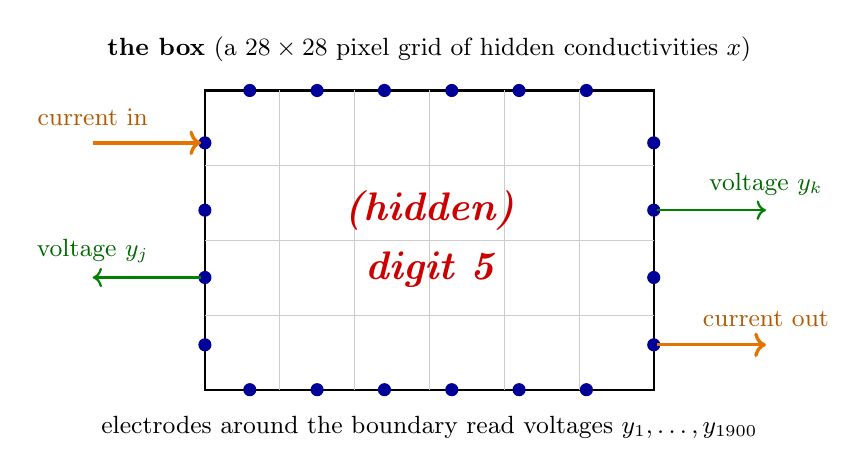
\begin{tikzpicture}[scale=0.95]
% box
\draw[thick] (0,0) rectangle (6,4);
% pixel grid (light)
\foreach \i in {1,...,5}{\draw[gray!40, very thin] (\i, 0) -- (\i, 4);}
\foreach \i in {1,2,3}{\draw[gray!40, very thin] (0, \i) -- (6, \i);}
% hidden digit (cartoon 5)
\node[red!80!black, font=\Large\bfseries] at (3,2.4) {\itshape (hidden)};
\node[red!80!black, font=\Large\bfseries] at (3,1.6) {\itshape digit 5};
% electrodes on the box
\foreach \x in {0.6, 1.5, 2.4, 3.3, 4.2, 5.1}{
  \filldraw[blue!60!black] (\x, 0) circle (0.08);
  \filldraw[blue!60!black] (\x, 4) circle (0.08);
}
\foreach \y in {0.6, 1.5, 2.4, 3.3}{
  \filldraw[blue!60!black] (0, \y) circle (0.08);
  \filldraw[blue!60!black] (6, \y) circle (0.08);
}
% current injection (top-left electrode): label sits above the arrow
\draw[->, very thick, orange!90!black] (-1.5, 3.3) -- (-0.05, 3.3);
\node[orange!70!black, font=\small] at (-1.5, 3.65) {current in};
% current out (right-bottom electrode): label sits above the arrow
\draw[->, very thick, orange!90!black] (6.05, 0.6) -- (7.5, 0.6);
\node[orange!70!black, font=\small] at (7.5, 0.95) {current out};
% voltage readouts
\draw[->, thick, green!50!black] (6.05, 2.4) -- (7.5, 2.4);
\node[green!40!black, font=\small] at (7.5, 2.75) {voltage $y_k$};
\draw[->, thick, green!50!black] (-0.05, 1.5) -- (-1.5, 1.5);
\node[green!40!black, font=\small] at (-1.5, 1.85) {voltage $y_j$};
% labels above and below the box
\node at (3, 4.55) {\small \textbf{the box} (a $28 \times 28$ pixel grid of hidden conductivities $x$)};
\node at (3, -0.5) {\small electrodes around the boundary read voltages $y_1, \ldots, y_{1900}$};
\end{tikzpicture}
\end{center}

The box is a $28\times 28$ grid. Each grid cell is one pixel of the
hidden image $x$, which encodes ``how easily electricity flows here.''
The little blue dots around the edge are electrodes, and the orange
arrows are one ``little experiment'' --- we push current in one
electrode and let it come out another. While that current flows, we
measure voltages at the other electrodes (green arrows). Over many such
experiments, we collect $1900$ voltage readings, which we stack into a
column vector $y$.

\textbf{Why does this even give us any information about the inside?}
Because electric current flows easily through high-conductivity material
and struggles through low-conductivity material. The pattern of voltages
at the edge depends on what's inside. A blob of high conductivity in the
middle ``soaks up'' current and produces a particular voltage pattern;
move the blob, and the pattern shifts. So the readings carry information
about the digit --- just a garbled, edge-only, blurred-out version of it.

\analogy{It's like a medical CT scanner that only has sensors on the
outside of your body. The sensors don't see the bones directly. They see
how X-rays bent on their way through. From those bending patterns,
software reconstructs an internal image. ERT is the electrical analog of
that.}

\section{Lesson 3: Why this is hard}

Two reasons.

\textbf{Reason 1: many different $x$'s give nearly the same $y$.} The
electrodes are far from the inside. A small feature inside the box
barely shows up at the edge, and several different inside-pictures
produce edge readings that differ only slightly. So if all we ask for
is ``find any $x$ with $F(x) \approx y_{\text{obs}}$,'' we get many
candidates, including ugly noise-looking pictures that fit the readings
to a few decimal places but look nothing like a digit.

\textbf{Reason 2: tiny errors in $y$ blow up in $x$.} Even if the
measurements are nearly perfect, the inverse map is so sensitive that
small noise in $y$ can cause wildly different reconstructions in $x$.

Both reasons say the same thing: pure data-fitting is not enough. We
need an extra rule that says ``the answer should also look like a real
digit, not like noise.'' That extra rule is called a \emph{prior}, and
choosing one is the whole game.

\analogy{If someone asks ``what is $2 + ? = 5$,'' the answer is $3$,
unique. But if someone asks ``what is $? + ? = 5$,'' the answer is any
pair that sums to 5. We need a second rule, like ``both numbers are
between 0 and 5,'' to narrow it down. The prior is that second rule.}

\section{Lesson 4: The rule for Project 2}

Project~1 used a particular prior: ``the answer is close to one of the
60{,}000 MNIST training digits.'' That worked, but it is a very strong
and very specific prior --- essentially a lookup table.

Project 2 says: \textbf{the prior must be a diffusion model}. A diffusion
model is a neural network that has learned what a digit looks like, by
practicing on lots of digits, and that can be used to generate fresh
digit-shaped images at random. Once we have one, we have to combine it
with our data $y_{\text{obs}}$ to recover the actual digit.

This is the whole assignment. The rest of this guide is about how to
take a diffusion model (which only knows about digits in the abstract)
and use it to recover the specific digit that produced $y_{\text{obs}}$.

\begin{intuition}
You can think of a diffusion model as a sketch artist who has practiced
drawing thousands of digits. Ask them to sketch a digit at random, they
can. Ask them ``which digit produced these specific 1900
measurements?'' and they have no idea --- they have not seen the
measurements. Our job is to combine the sketch artist with the
measurements so they together produce the right digit.
\end{intuition}

%==============================================================
\part*{Part II --- What is a diffusion model?}
\addcontentsline{toc}{section}{Part II --- What is a diffusion model?}
%==============================================================

\section{Lesson 5: The strange but useful idea}

A diffusion model is trained on one weird idea: take a clean picture,
slowly destroy it with random noise until it is pure static, and train
a neural network to \emph{undo} that destruction one tiny step at a
time.

Why does this teach the network anything useful? Because in order to
undo the destruction one step at a time, the network has to learn what
a slightly-less-noisy version of a digit picture looks like. After lots
of practice on lots of training digits, it has effectively learned
``what a digit looks like, in the presence of noise.'' That turns out
to be enough to do everything we want.

We will spend Lessons 6 through 13 building this up carefully. Take it
slow. The math is not hard, but it has a lot of small moving parts, and
each one shows up in later lessons.

\section{Lesson 6: The forward chain, one step at a time}

Pick a clean digit. We will call it $x_0$. The subscript $0$ means
``zero noise, totally clean.'' Think of $x_0$ as a $28\times 28$ grid
of numbers between $0$ (black background) and $1$ (bright stroke). Don't
worry about its exact pixel values; just hold the picture in your head.

We pick a tiny number $\beta_1$. (The Greek letter ``beta'' is just a
name for it.) In practice $\beta_1$ is something like $10^{-4}$. We then
build a slightly-noisier version of the picture, called $x_1$:
\[
x_1 \;=\; \sqrt{1 - \beta_1}\;x_0 \;+\; \sqrt{\beta_1}\;\varepsilon_1.
\]

Let me unpack every piece of that line:
\begin{itemize}[leftmargin=2em]
\item $\varepsilon_1$ is a $28\times 28$ grid of random numbers drawn
  from a standard Gaussian (bell curve, mean 0, variance 1). Each pixel
  of $\varepsilon_1$ is an independent random draw. So $\varepsilon_1$
  on its own looks like pure TV-snow static.
\item The first term, $\sqrt{1 - \beta_1}\,x_0$, is the clean picture
  shrunk by a tiny amount. Because $\beta_1$ is small,
  $\sqrt{1 - \beta_1}$ is very close to $1$, so this is almost just
  $x_0$ itself.
\item The second term, $\sqrt{\beta_1}\,\varepsilon_1$, is the static
  $\varepsilon_1$ scaled down by a small factor. Because $\beta_1$ is
  small, $\sqrt{\beta_1}$ is also small, so this contributes just a
  sprinkle of noise.
\item Add the two together: we get $x_1$, the original picture with a
  tiny bit of noise smeared on top.
\end{itemize}

So step 1 of the forward chain takes the clean picture and adds a sprinkle
of noise. The picture still looks essentially identical to $x_0$ at this
point.

Step 2 does the same thing again, with a slightly bigger $\beta_2$:
\[
x_2 \;=\; \sqrt{1 - \beta_2}\;x_1 \;+\; \sqrt{\beta_2}\;\varepsilon_2,
\]
with a fresh random $\varepsilon_2$. And then step 3, step 4, all the
way up to step $T = 1000$. The $\beta_t$'s grow as $t$ grows, so the
noise added per step gets bigger. By step $1000$, the picture is
\emph{utterly gone} --- $x_{1000}$ is just pure Gaussian static,
indistinguishable from what you'd get if you skipped the digit entirely.

\analogy{Imagine staring at a perfectly clear window. Every minute,
someone breathes on it a little. After one breath, you can still see
through. After 10 breaths, hazy. After 1000 breaths, it's just fog and
you can't see anything. The forward chain is exactly that: the ``view''
is a digit and each ``breath'' is one step of noise.}

\begin{key}
The \emph{forward chain} is a $1000$-step process that turns a clean
digit picture into pure noise. Each step adds a tiny sprinkle.
\end{key}

\section{Lesson 7: A picture of the forward chain}

Let's actually look at what this destruction process looks like. Below
is one MNIST digit (a 5) shown at six different points along the forward
chain.

\begin{center}
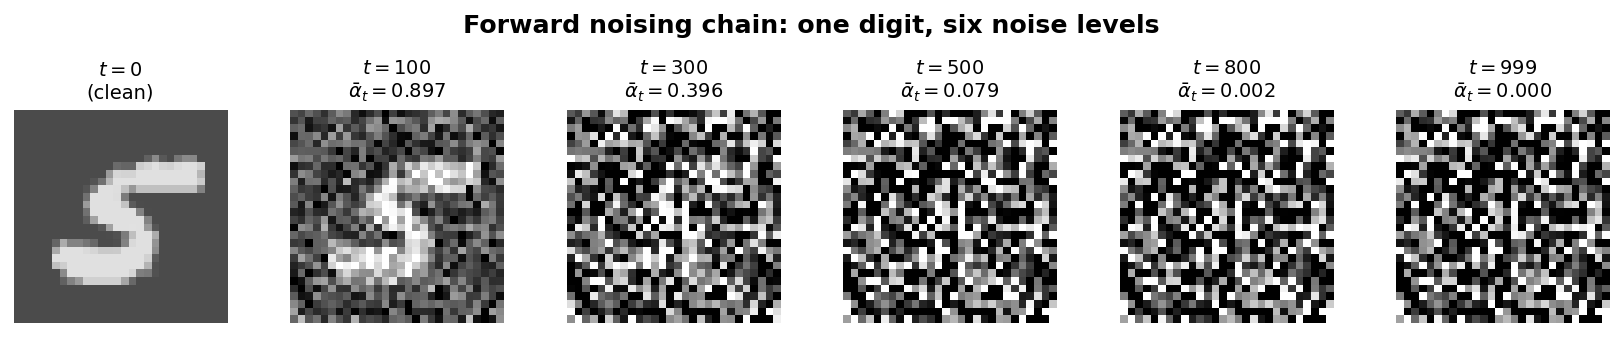
\includegraphics[width=0.99\textwidth]{fig02_forward_chain.png}
\end{center}

\begin{itemize}[leftmargin=2em]
\item At $t = 0$ (clean), it's just the digit.
\item At $t = 100$, you can already see noise sprinkled on the
  background, but the 5 is still obvious.
\item At $t = 300$, the noise has gotten substantial. You can
  \emph{barely} make out the 5 if you squint.
\item At $t = 500$, the 5 is mostly buried under noise. A neural network
  could still pick it out, but a human is having a hard time.
\item At $t = 800$, almost nothing is left.
\item At $t = 999$, just static. The original 5 is unrecoverable by eye.
\end{itemize}

The number $\bar\alpha_t$ under each panel (we'll define it formally in
the next lesson) measures ``how much of the original is left.'' At
$t=0$, $\bar\alpha_t = 1$ (all of it). At $t=999$, $\bar\alpha_t = 0.0005$
(essentially none of it).

This is what the forward chain looks like for one digit. For training,
we run the chain on every training digit, getting a noisy version of
every digit at every noise level. That's a lot of (noisy digit, noise
level) pairs, and that's the training data for the network.

\section{Lesson 8: A shortcut --- the closed-form noising formula}

We do not actually have to run all 1000 steps to know what $x_t$ looks
like. There is a one-line shortcut.

Define
\[
\bar\alpha_t \;:=\; \prod_{s=1}^{t}\,(1 - \beta_s).
\]
The symbol $\prod$ just means ``multiply these all together.'' So
$\bar\alpha_t$ is the product $(1 - \beta_1)(1 - \beta_2)\cdots(1 -
\beta_t)$. It's the cumulative version of the per-step shrink factor.

\textbf{Numerical example.} Say $\beta_t$ is constant at $10^{-4}$ for
the first 100 steps. Then
\[
\bar\alpha_{100} \;=\; (1 - 10^{-4})^{100} \;\approx\; 0.99.
\]
After 100 steps, about $99\%$ of the original signal remains. That
matches what we see in Figure above: at $t = 100$, the digit is still
very clearly visible.

After 1000 steps, with the schedule the model actually uses (growing
$\beta$'s), $\bar\alpha_{1000}$ is around $5 \times 10^{-4}$. Almost no
signal left.

\textbf{The shortcut.} Instead of running $t$ small steps, you can write
\[
\boxed{\;\; x_t \;=\; \sqrt{\bar\alpha_t}\;x_0 \;+\; \sqrt{1 - \bar\alpha_t}\;\varepsilon, \quad \varepsilon \sim \mathcal{N}(0, I). \;\;}
\]

That is: $x_t$ is just $x_0$ shrunk by $\sqrt{\bar\alpha_t}$, plus
\emph{one} Gaussian noise sample scaled by $\sqrt{1 - \bar\alpha_t}$.
No chain of 1000 steps required. (Why is this allowed? Because adding
independent Gaussians at every step still gives you a Gaussian at the
end, with a known variance.)

\begin{itemize}[leftmargin=2em]
\item When $t = 0$: $\bar\alpha_0 = 1$, so $x_0 = 1\cdot x_0 + 0\cdot
  \varepsilon = x_0$. Clean, as expected.
\item When $t = T = 1000$: $\bar\alpha_T \approx 0$, so $x_T \approx
  0\cdot x_0 + 1\cdot \varepsilon = \varepsilon$. Pure noise, as expected.
\item In between, $\bar\alpha_t$ slides from $1$ down to $0$. So
  $\sqrt{\bar\alpha_t}$ slides from $1$ down to $0$ (the original fades
  out) and $\sqrt{1 - \bar\alpha_t}$ slides from $0$ up to $1$ (the
  noise takes over).
\end{itemize}

\begin{intuition}
$\bar\alpha_t$ is the ``how much of the original is still here'' at
step $t$. It is the single number that captures where we are in the
forward chain. You will see this letter on almost every page.
\end{intuition}

\section{Lesson 9: What the network does --- inputs and outputs}

The forward chain is just math. The reverse direction --- recovering
the digit from a noisy version --- is what we train a neural network to
do.

\textbf{The contract.} The network takes two inputs --- a noisy picture
and which step we are at --- and produces one output --- a guess at the
noise that was added.

\begin{center}
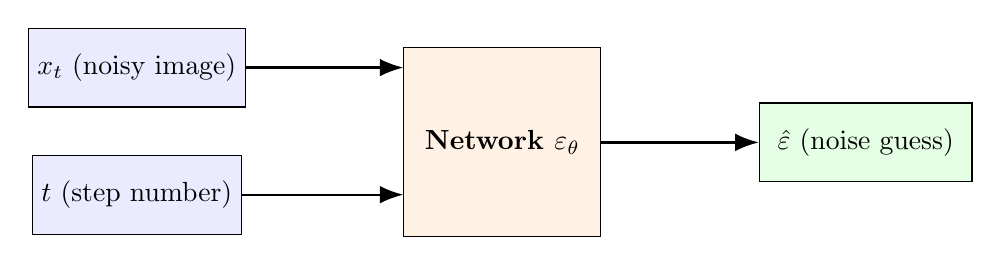
\begin{tikzpicture}[node distance=1.3cm]
\node[draw, rectangle, minimum width=2.3cm, minimum height=1cm, fill=blue!8] (input1) {\(x_t\) (noisy image)};
\node[draw, rectangle, minimum width=2.3cm, minimum height=1cm, fill=blue!8, below=0.6cm of input1] (input2) {\(t\) (step number)};
\node[draw, rectangle, minimum width=2.5cm, minimum height=2.4cm, fill=orange!10, right=2cm of input1, yshift=-0.95cm] (net) {\bfseries Network \(\varepsilon_\theta\)};
\node[draw, rectangle, minimum width=2.7cm, minimum height=1cm, fill=green!10, right=2cm of net] (output) {\(\hat\varepsilon\) (noise guess)};
\draw[-{Latex[length=3mm]}, thick] (input1.east) -- (net.west |- input1);
\draw[-{Latex[length=3mm]}, thick] (input2.east) -- (net.west |- input2);
\draw[-{Latex[length=3mm]}, thick] (net.east) -- (output.west);
\end{tikzpicture}
\end{center}

We write the network as $\varepsilon_\theta(x_t, t)$. The little
$\theta$ subscript is just a reminder that the network has internal
weights that we have to learn during training; once it's trained you
can ignore $\theta$ and just call it ``the network.''

The output $\hat\varepsilon$ has the same shape as $x_t$ (so $28\times
28$). It's the network's guess at the noise sample that was used to
build $x_t$ from $x_0$.

\textbf{Why predict the noise rather than the clean image?} Predicting
noise turns out to be easier and more numerically stable in practice.
But it doesn't really matter --- once you can predict the noise, you
can also recover the clean image, with one line of algebra. (Lesson
11.)

\textbf{What does the network look like inside?} A so-called U-Net:
some convolutional layers that progressively compress the image, then
some that expand back to $28\times 28$. The architecture details don't
matter for our purposes. What matters is the contract above.

\section{Lesson 10: Training the network}

We train the network so that for any clean picture, any step $t$, and
any noise sample $\varepsilon$, it correctly predicts $\varepsilon$.
The training loop has six steps:

\begin{center}
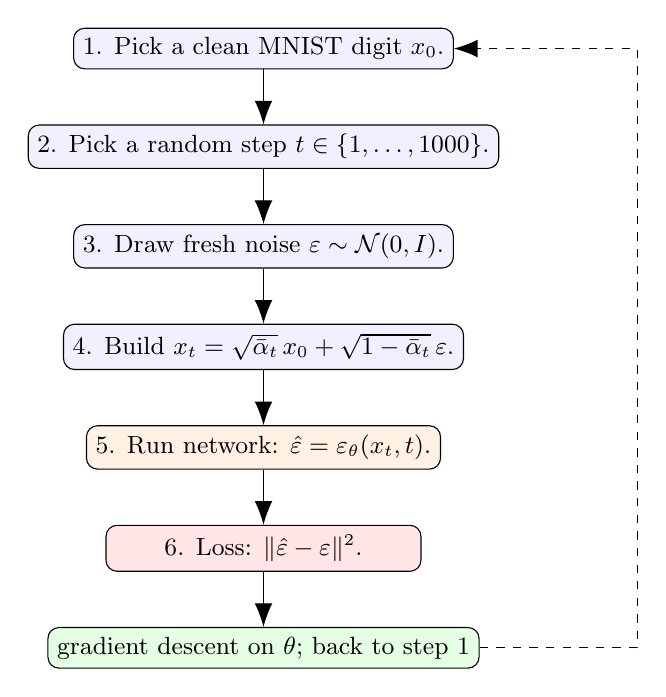
\begin{tikzpicture}[node distance=0.7cm, every node/.style={font=\small}]
\node[draw, rectangle, rounded corners, fill=blue!6, minimum width=4cm] (a) {1. Pick a clean MNIST digit \(x_0\).};
\node[draw, rectangle, rounded corners, fill=blue!6, minimum width=4cm, below=of a] (b) {2. Pick a random step \(t \in \{1, \ldots, 1000\}\).};
\node[draw, rectangle, rounded corners, fill=blue!6, minimum width=4cm, below=of b] (c) {3. Draw fresh noise \(\varepsilon \sim \mathcal{N}(0, I)\).};
\node[draw, rectangle, rounded corners, fill=blue!6, minimum width=4cm, below=of c] (d) {4. Build \(x_t = \sqrt{\bar\alpha_t}\,x_0 + \sqrt{1-\bar\alpha_t}\,\varepsilon\).};
\node[draw, rectangle, rounded corners, fill=orange!10, minimum width=4cm, below=of d] (e) {5. Run network: \(\hat\varepsilon = \varepsilon_\theta(x_t, t)\).};
\node[draw, rectangle, rounded corners, fill=red!10, minimum width=4cm, below=of e] (f) {6. Loss: \(\|\hat\varepsilon - \varepsilon\|^2\).};
\node[draw, rectangle, rounded corners, fill=green!10, minimum width=4cm, below=of f] (g) {gradient descent on \(\theta\); back to step 1};
\draw[-{Latex[length=3mm]}] (a) -- (b);
\draw[-{Latex[length=3mm]}] (b) -- (c);
\draw[-{Latex[length=3mm]}] (c) -- (d);
\draw[-{Latex[length=3mm]}] (d) -- (e);
\draw[-{Latex[length=3mm]}] (e) -- (f);
\draw[-{Latex[length=3mm]}] (f) -- (g);
\draw[-{Latex[length=3mm]}, dashed] (g.east) -- ++(2,0) |- (a.east);
\end{tikzpicture}
\end{center}

After many passes through the training data, the network gets good at
predicting noise from any (noisy-picture, step) pair.

Notice the cost of training data: zero. For each clean training digit
$x_0$ we can synthesize $1000$ training pairs (one per possible $t$).
We never had to collect ``ground-truth pairs'' from somewhere; the
forward chain manufactures them on demand.

\begin{aside}
The base prior in Lessons 18--35 is the pretrained MNIST DDPM
\texttt{1aurent/ddpm-mnist} on Hugging Face (about $1$ million internal
weights), trained this way on standard MNIST for a few hours on one GPU.
We downloaded that one and fine-tuned it on rotated MNIST. In Lesson 39
we train a bigger $6$-million-parameter UNet from scratch using exactly
the loop above (with EMA weights), and in Lesson 40 a class-conditional
variant. The training procedure is identical; only the architecture and
the data pairing change.
\end{aside}

\section{Lesson 11: Tweedie's formula --- recovering the clean image from the noise guess}

OK here is where we cash in. The network predicts the \emph{noise}.
What we really want is a guess at the \emph{clean image} that the noise
was added to. The good news is: if we have one, algebra gives us the
other.

Go back to the closed-form noising formula:
\[
x_t \;=\; \sqrt{\bar\alpha_t}\;x_0 \;+\; \sqrt{1 - \bar\alpha_t}\;\varepsilon.
\]
This is a relationship between three things: $x_t$ (which we see),
$x_0$ (what we want), and $\varepsilon$ (which the network can guess).

Pretend the network's guess $\hat\varepsilon$ is exact, and \emph{solve}
the formula for $x_0$. Step by step.

\textbf{Step 1.} Start with
\[
x_t \;=\; \sqrt{\bar\alpha_t}\;x_0 \;+\; \sqrt{1 - \bar\alpha_t}\;\hat\varepsilon.
\]

\textbf{Step 2.} Subtract $\sqrt{1 - \bar\alpha_t}\,\hat\varepsilon$ from
both sides to isolate the term containing $x_0$:
\[
x_t \;-\; \sqrt{1 - \bar\alpha_t}\;\hat\varepsilon
\;=\; \sqrt{\bar\alpha_t}\;x_0.
\]

\textbf{Step 3.} Divide both sides by $\sqrt{\bar\alpha_t}$ to solve
for $x_0$ alone:
\[
\frac{x_t \;-\; \sqrt{1 - \bar\alpha_t}\;\hat\varepsilon}{\sqrt{\bar\alpha_t}}
\;=\; x_0.
\]

That's it. The thing on the left is the network's implicit guess at
the clean image, given $x_t$ and the network's noise prediction. We
give it its own name $\hat x_0$:
\[
\boxed{\;\; \hat x_0(x_t, t) \;:=\;
\frac{x_t \;-\; \sqrt{1 - \bar\alpha_t}\;\varepsilon_\theta(x_t, t)}{\sqrt{\bar\alpha_t}}. \;\;}
\]

This is called \textbf{Tweedie's formula} (after Maurice Tweedie). There
is a deeper statistical reason why it's exact in expectation, but for
our purposes it is just ``the noising formula solved for $x_0$, using
the network's noise prediction as a stand-in for the unknown $\varepsilon$.''

\begin{key}
$\hat x_0$ is the \emph{denoiser as oracle}. At any moment along the
noisy chain, ask the network for its $\hat x_0$ and you get a guess
at the underlying clean digit. We will call this oracle constantly.
\end{key}

\section{Lesson 12: A picture of Tweedie's estimates}

The Tweedie formula is mathematical, but its output is a literal image
we can look at. Below, the top row shows $x_t$ at four different noise
levels (the noisy inputs). The bottom row shows the corresponding
$\hat x_0$ (the network's guess at the clean image).

\begin{center}
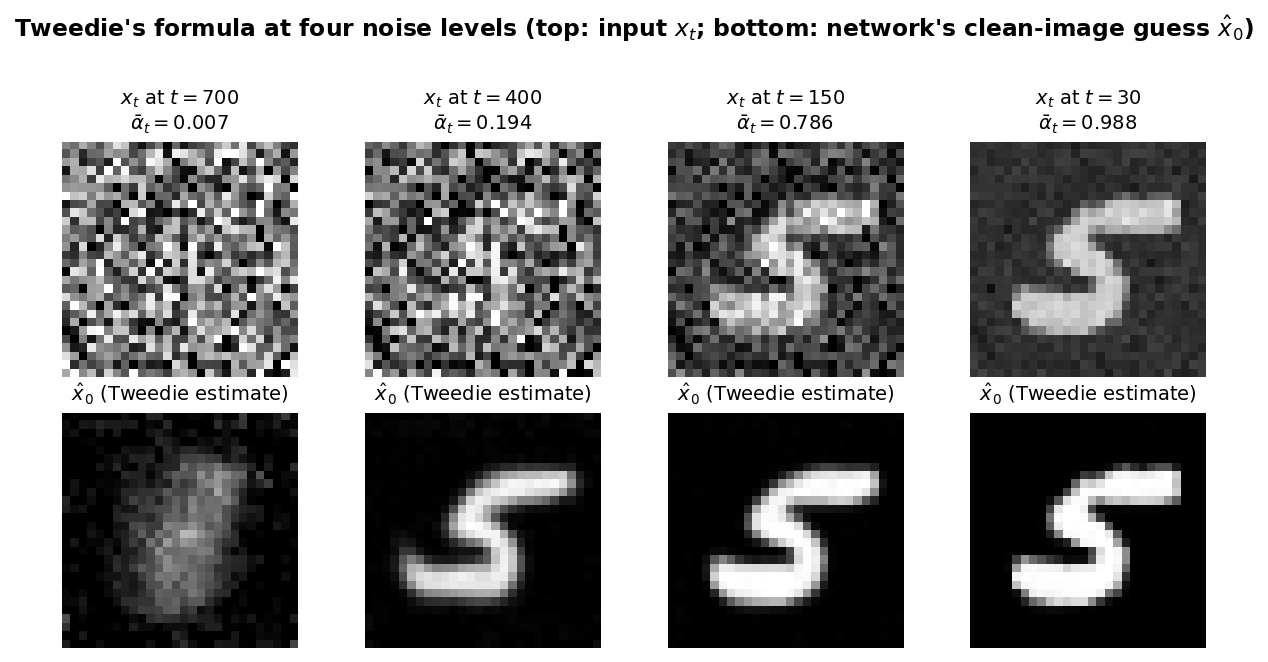
\includegraphics[width=0.95\textwidth]{fig05_tweedie_strip.png}
\end{center}

What you should see:

\begin{itemize}[leftmargin=2em]
\item At $t = 700$ (top-left): $x_t$ is mostly noise (only a faint
  shape is visible). The network's $\hat x_0$ is a blurry but
  recognizable 5. The network has committed to ``a 5 is in here
  somewhere'' but the strokes are fuzzy.
\item At $t = 400$: $x_t$ is half-noise, half-digit. The Tweedie
  estimate is a clearer 5, with strokes sharpening up.
\item At $t = 150$: $x_t$ is mostly clean with some grain. The Tweedie
  estimate is essentially the clean digit.
\item At $t = 30$: $x_t$ is almost clean; Tweedie just refines it.
\end{itemize}

The Tweedie estimate gets sharper as we move from high $t$ to low $t$.
At high $t$ it's a fuzzy commitment; at low $t$ it's a confident
prediction. \emph{This is the lever PnP-DM is going to pull.} Whenever
we want the network's current best guess at the clean digit, we call
Tweedie at the current noise level.

\section{Lesson 13: Generating a fresh digit (no data involved)}

To round out our understanding of diffusion models, let's see how to
use one for its original purpose: generating fresh digits at random,
without any data.

The recipe is just the reverse chain:
\begin{enumerate}[leftmargin=2em]
\item Start at $x_T \sim \mathcal{N}(0, I)$ --- pure noise.
\item For $t = T, T-1, \ldots, 1$:
  \begin{itemize}[leftmargin=1.5em]
    \item Run the network on $(x_t, t)$ to get $\hat\varepsilon$.
    \item Compute $\hat x_0$ via Tweedie.
    \item Use a known formula to combine $x_t$ and $\hat x_0$ into a
      slightly-less-noisy next picture $x_{t-1}$. Also inject a tiny
      bit of fresh noise so different runs produce different digits.
  \end{itemize}
\item When $t$ reaches $0$, output $x_0$.
\end{enumerate}

If we run this whole loop with one random starting noise, we get one
random fresh digit. Run it again with new noise, get a different
digit. The outputs are clearly digits (the network learned what digits
look like), but they are random --- none of them is \emph{a particular}
digit we asked for. We will see actual unconditional samples from our
(fine-tuned) diffusion model later in Part IV when we compare it
against the pretrained version.

\textbf{None of this used the data.} We just generated random fresh
digits. For our inverse problem we need to do more: we need the chain
to commit to ``the digit that actually produced $y_{\text{obs}}$,''
not some random digit. That requires combining the diffusion model with
the data, which is what Part III is about.

%==============================================================
\part*{Part III --- Bayes and posterior sampling}
\addcontentsline{toc}{section}{Part III --- Bayes and posterior sampling}
%==============================================================

\section{Lesson 14: Bayes' rule, with a one-number example}

Forget images for a moment. Suppose we are trying to estimate a single
number $x$. We have one piece of data $y$ that depends on $x$ but is
noisy, and we have a prior belief about what $x$ usually looks like.

Bayes' rule combines those two:
\[
p(x \mid y) \;\propto\; p(y \mid x) \;\cdot\; p(x).
\]
\textbf{Translation in plain English:} ``the probability that the true
answer is $x$, given that we observed $y$, is proportional to (the
chance of seeing $y$ if the true answer were $x$) times (the prior
chance that $x$ is plausible).''

The two pieces:
\begin{itemize}[leftmargin=2em]
\item $p(y \mid x)$ is called the \emph{likelihood}. It comes from the
  measurement physics. In our problem the physics says $y \approx F(x)$,
  with Gaussian measurement noise, so $p(y \mid x)$ is a bell curve
  centered at $F(x)$.
\item $p(x)$ is the \emph{prior}. It encodes ``what $x$ usually looks
  like, before any data.'' For Project 2, this is what the diffusion
  model represents.
\end{itemize}

\textbf{A concrete one-number example.} Suppose $x$ is the height of an
adult in inches. Our prior says heights are roughly $\mathcal{N}(67, 4^2)$
(mean $67$, standard deviation $4$). We measure $y = 80$ inches with a
ruler that has noise standard deviation $1$.

Bayes' rule asks: \emph{what is the probability that the true height is $x$?}
If we ignored the prior, we'd say $x \approx 80$ (just the measurement).
If we ignored the data, we'd say $x \approx 67$ (just the prior). Bayes
combines them with weights proportional to each one's precision.

For two Gaussians, the posterior is also Gaussian, with mean
\[
\mu_{\text{post}} \;=\;
\frac{\mu_p / \sigma_p^2 + \mu_l / \sigma_l^2}{1/\sigma_p^2 + 1/\sigma_l^2}
\;=\;
\frac{67/16 + 80/1}{1/16 + 1/1}
\;=\;
\frac{4.1875 + 80}{1.0625}
\;\approx\;
79.2.
\]

So the posterior peak is at $79.2$ inches --- pulled mostly toward the
data ($80$) because the ruler's $1$-inch noise is tight, with only a
small tug toward the prior ($67$) because the prior's $4$-inch spread is
wide. Whichever source has smaller variance gets more say in the
posterior, and here the data wins.

\section{Lesson 15: A picture of Bayes in 1D}

Same math, drawn as three bell curves on one axis:

\begin{center}
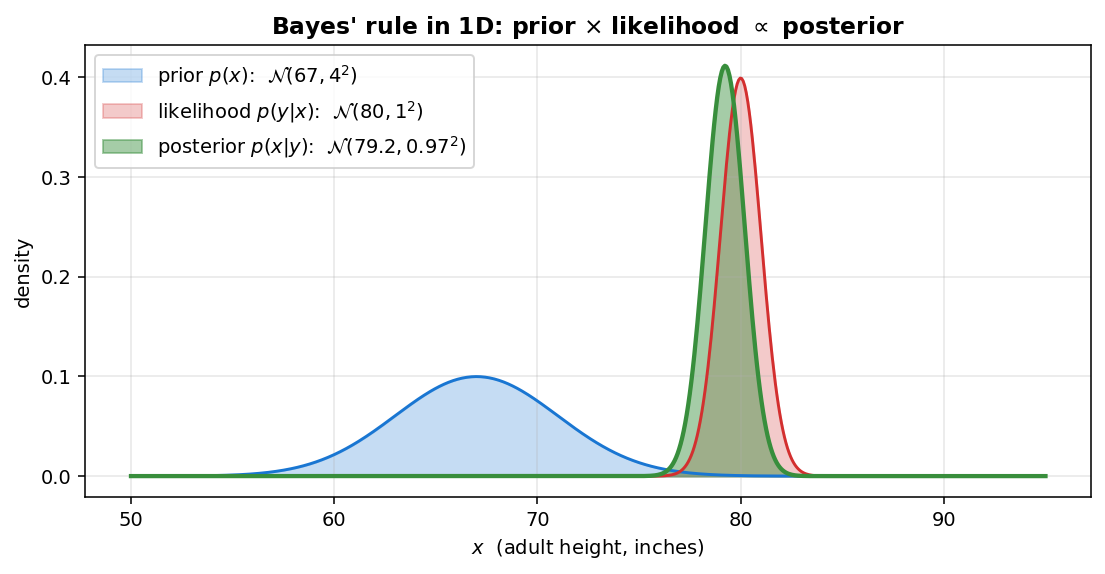
\includegraphics[width=0.95\textwidth]{fig07_bayes_1d.png}
\end{center}

Read the three curves:
\begin{itemize}[leftmargin=2em]
\item Blue (prior, $p(x)$): broad, peaked at $67$, spread out over
  $\sim 4$ inches. ``Adults are usually around 67, give or take.''
\item Red (likelihood, $p(y \mid x)$ for $y = 80$): narrow, peaked at
  $80$. ``The ruler said 80, plus or minus 1.''
\item Green (posterior, $p(x \mid y)$): the product of the two,
  appropriately normalized. Peaked at $79.2$, much tighter than the
  prior.
\end{itemize}

The posterior is \emph{narrower} than either factor alone. Combining
two beliefs always sharpens (or at least never widens). And the
posterior peak is between the prior peak and the likelihood peak,
weighted by precision.

\textbf{For our problem.} Same picture, just in $784$ dimensions. The
prior $p(x)$ is what the diffusion model represents (peaked on
digit-shaped images). The likelihood $p(y \mid x)$ is peaked on images
whose $F(x)$ matches $y_{\text{obs}}$. The posterior $p(x \mid y_{\text{obs}})$
is peaked on images that simultaneously look like digits and match the
data. That is what we want to sample from.

\section{Lesson 16: ``Sampling'' from the posterior (vs maximizing)}

We don't just want one estimate of $x$. We want \emph{samples} from
$p(x \mid y_{\text{obs}})$. Why?

Because for ill-posed problems the posterior can have several modes ---
several distinct images that all reasonably explain the data. If we
draw samples and they all look like 5s, we know the answer is a 5 with
high confidence. If they split between 5s and 6s, the data was
genuinely ambiguous and we should report that.

For Project 2, our pipeline draws 32 samples (call them
$x^{(1)}, \ldots, x^{(32)}$). At the end we keep the one with the
smallest data misfit $\norm{F(x^{(i)}) - y_{\text{obs}}}^2$. That's our
final pre-polish answer.

\begin{intuition}
Sampling reveals ambiguity. Maximizing (just finding the one most
probable image) hides it. We sample first, then optimize.
\end{intuition}

\section{Lesson 17: A first attempt --- DPS, and why it isn't enough}

We have a network that does \emph{unconditional} sampling (Lesson 13).
We have a formula for $p(y \mid x)$. How do we combine them so the
network samples \emph{conditionally} on $y_{\text{obs}}$?

The simplest idea, called \emph{Diffusion Posterior Sampling (DPS)},
is: at every step of the reverse chain, add a small extra nudge in the
direction that makes the data fit better. That nudge uses the gradient
of $\norm{F(\hat x_0) - y_{\text{obs}}}^2$ with respect to $x_t$, which
works out (using the chain rule and Tweedie) to a small multiple of
$J^\top(F(\hat x_0) - y_{\text{obs}})$, where $J$ is the ERT Jacobian.

In words: at every reverse step, the data tugs the candidate one
slightly more toward fitting $y_{\text{obs}}$, while the network's
denoising step tugs it slightly more toward looking like a digit.

\textbf{Why this isn't enough for us.} The two tugs happen on the same
variable at the same time. They compromise on every step. For our
specific problem, the data tug is too weak to overcome the prior tug
within the 100 or so reverse steps we have, and the chain commits to
the wrong digit. Empirically, with DPS we couldn't recover digit 5 even
once, across many random seeds. Four of five chains converged to a 4;
the fifth converged to a 6.

We also tried three other diffusion-based recipes before landing on
the method in the rest of this guide:
\begin{itemize}[leftmargin=2em]
\item \textbf{DAPS} (Decoupled Annealing Posterior Sampling, Zhang et al.,
  CVPR 2025). The diffusion model is responsible for class and shape;
  a separate Langevin step is responsible for fitting the data. Cleaner
  separation than DPS, but still committed to a 4 most runs.
\item \textbf{DAPS + classifier vote.} Run DAPS, then ask a separately
  trained MNIST classifier to pick the digit class. The classifier voted
  ``4'' too --- because the recovered images really did look like 4s.
\item \textbf{DAPS + template retrieval.} Run DAPS, then snap the
  result to the nearest training image. The nearest training image was
  always an upright digit, but the competition truth is tilted by 7.5
  degrees. The retrieved template was the right class for some seeds
  but at the wrong pose, and the polish could not unfold it.
\end{itemize}

All four recipes share one structural flaw: a weak per-step data tug
that cannot pull the chain out of whatever upright-digit basin the
prior settled into. DAPS already separates the prior step from the
data step (a strict improvement over DPS in that respect), but its
data step is still a sequence of small Langevin gradient updates, so
it inherits the same weakness.

The fix --- and the actual method we use --- has two parts. \emph{First},
introduce a second variable so each pull acts on its own variable
alone (the two are glued together with a soft penalty). \emph{Second},
make the data update use the full Jacobian via a small Gauss-Newton
solve, so one update does the work of dozens of gradient steps. The
combination is called PnP-DM (Wu et al., NeurIPS 2024) and the rest of
this guide is how to actually run it.

\begin{center}
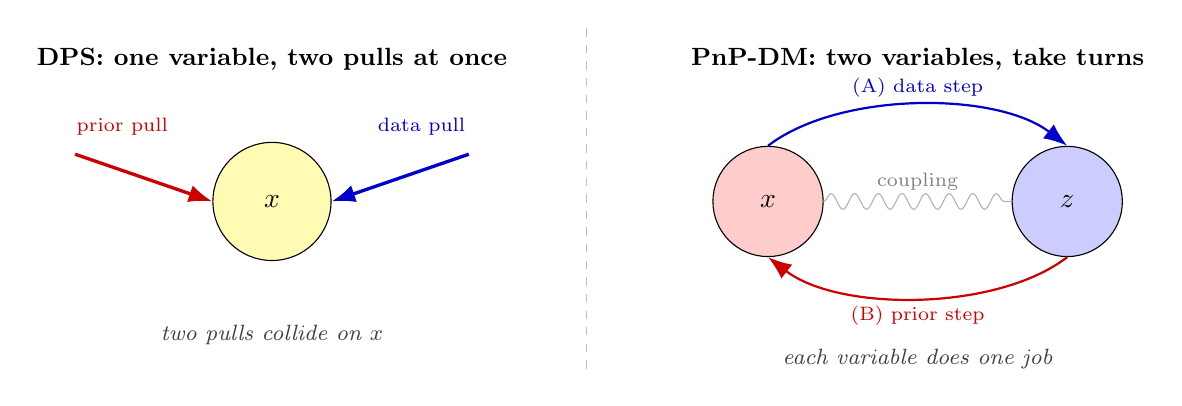
\begin{tikzpicture}
% ---- LEFT: DPS ----
\node[font=\small\bfseries] at (-2.5, 2.4) {DPS: one variable, two pulls at once};
\node[draw, circle, fill=yellow!30, minimum size=1.5cm] (x) at (-2.5, 0.6) {\(x\)};
\draw[-{Latex[length=3mm]}, very thick, red!80!black] (-5.0, 1.2) -- (x.west);
\node[red!80!black, font=\scriptsize] at (-4.4, 1.55) {prior pull};
\draw[-{Latex[length=3mm]}, very thick, blue!80!black] (-0.0, 1.2) -- (x.east);
\node[blue!80!black, font=\scriptsize] at (-0.6, 1.55) {data pull};
\node[font=\footnotesize\itshape, gray!50!black] at (-2.5, -1.1) {two pulls collide on $x$};
% ---- vertical divider ----
\draw[gray!50, dashed] (1.5, 2.8) -- (1.5, -1.6);
% ---- RIGHT: PnP-DM ----
\node[font=\small\bfseries] at (5.7, 2.4) {PnP-DM: two variables, take turns};
\node[draw, circle, fill=red!20, minimum size=1.4cm] (xR) at (3.8, 0.6) {\(x\)};
\node[draw, circle, fill=blue!20, minimum size=1.4cm] (zR) at (7.6, 0.6) {\(z\)};
% data step: x -> z (upper arc)
\draw[-{Latex[length=3mm]}, thick, blue!80!black]
  (xR.north) .. controls (4.7, 2.0) and (6.7, 2.0) .. (zR.north);
\node[blue!80!black, font=\scriptsize] at (5.7, 2.05) {(A) data step};
% prior step: z -> x (lower arc)
\draw[-{Latex[length=3mm]}, thick, red!80!black]
  (zR.south) .. controls (6.7, -0.8) and (4.7, -0.8) .. (xR.south);
\node[red!80!black, font=\scriptsize] at (5.7, -0.85) {(B) prior step};
% coupling between them (wavy middle line)
\draw[gray!60, decorate, decoration={snake, amplitude=1mm, segment length=3mm}]
  (xR.east) -- (zR.west);
\node[font=\scriptsize, gray] at (5.7, 0.85) {coupling};
\node[font=\footnotesize\itshape, gray!50!black] at (5.7, -1.4) {each variable does one job};
\end{tikzpicture}
\end{center}

This trick has a name --- \emph{variable splitting} --- and the resulting
sampler is called PnP-DM. Part IV is about how to actually run it.

%==============================================================
\part*{Part IV --- PnP-DM: the actual method}
\addcontentsline{toc}{section}{Part IV --- PnP-DM: the actual method}
%==============================================================

\section{Lesson 18: The variable-splitting setup}

We introduce a second variable $z$. It has the same shape as $x$ (a
$28 \times 28$ image). The trick is that we will give $z$ and $x$
different jobs:
\begin{itemize}[leftmargin=2em]
\item $x$ has to look like a digit (only the prior touches it).
\item $z$ has to fit the measurements (only the likelihood touches it).
\item $z$ and $x$ are softly coupled, so they end up agreeing.
\end{itemize}

Then we alternate updating them. While we hold $x$ fixed and update $z$,
the data step doesn't have to worry about the prior. While we hold $z$
fixed and update $x$, the prior step doesn't have to worry about the
data. Each update is clean.

Mathematically, we write down a joint distribution over $(x, z)$ that
factors into three pieces:
\[
p(x, z \mid y_{\text{obs}})
\;\propto\;
\underbrace{p(y_{\text{obs}} \mid z)}_{\text{data sees }z}
\;\cdot\;
\underbrace{\mathcal{N}(z \mid x,\; \sigma_n^2 I)}_{\text{soft coupling}}
\;\cdot\;
\underbrace{p(x)}_{\text{prior sees }x}.
\]

The first factor: the data depends \emph{only on $z$}, never directly
on $x$. The third factor: the prior depends \emph{only on $x$}, never
directly on $z$. The middle factor is a Gaussian centered at $x$ with
spread $\sigma_n$, saying ``$z$ should be close to $x$, give or take
$\sigma_n$.'' That's the glue.

\begin{intuition}
$\sigma_n$ is the leash length between $z$ and $x$. Large $\sigma_n$:
loose leash, each variable explores freely. Small $\sigma_n$: tight
leash, they have to agree. We will anneal $\sigma_n$ from large at the
start (about $1$) down to small at the end (about $0.05$).
\end{intuition}

\section{Lesson 19: One iteration of PnP-DM, in pictures}

The algorithm alternates two updates per iteration. Visually:

\begin{center}
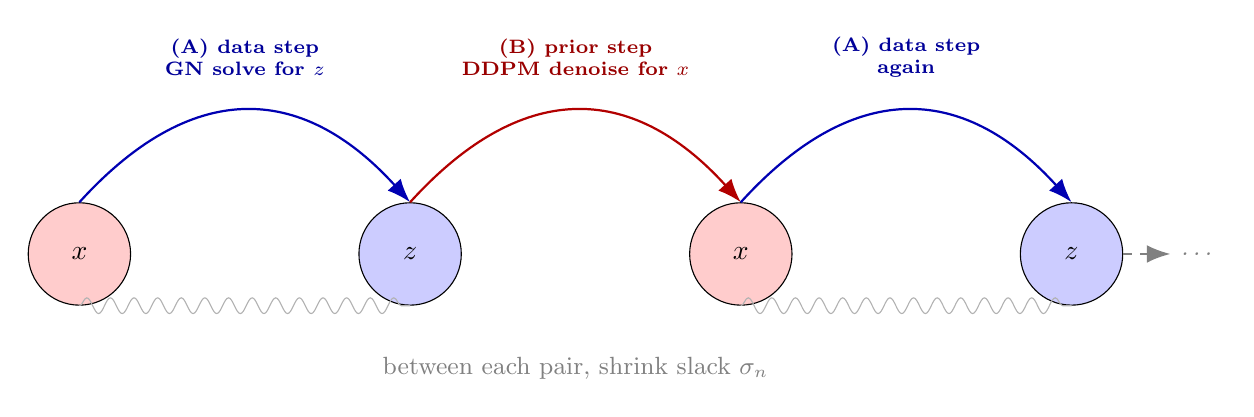
\begin{tikzpicture}
\node[draw, circle, fill=red!20, minimum size=1.3cm] (x1) at (0, 0) {\(x\)};
\node[draw, circle, fill=blue!20, minimum size=1.3cm] (z1) at (4.2, 0) {\(z\)};
\node[draw, circle, fill=red!20, minimum size=1.3cm] (x2) at (8.4, 0) {\(x\)};
\node[draw, circle, fill=blue!20, minimum size=1.3cm] (z2) at (12.6, 0) {\(z\)};
% Each arc has its own two-line label above, well separated.
\draw[-{Latex[length=3mm]}, thick, blue!70!black] (x1.north)
  .. controls (1.4, 2.2) and (2.8, 2.2) .. (z1.north);
\node[blue!60!black, font=\scriptsize\bfseries, align=center] at (2.1, 2.5)
  {(A) data step\\GN solve for \(z\)};
\draw[-{Latex[length=3mm]}, thick, red!70!black] (z1.north)
  .. controls (5.6, 2.2) and (7.0, 2.2) .. (x2.north);
\node[red!60!black, font=\scriptsize\bfseries, align=center] at (6.3, 2.5)
  {(B) prior step\\DDPM denoise for \(x\)};
\draw[-{Latex[length=3mm]}, thick, blue!70!black] (x2.north)
  .. controls (9.8, 2.2) and (11.2, 2.2) .. (z2.north);
\node[blue!60!black, font=\scriptsize\bfseries, align=center] at (10.5, 2.5)
  {(A) data step\\again};
\draw[-{Latex[length=3mm]}, thick, gray, dashed] (z2.east) -- ++(0.6,0)
  node[right, font=\small\itshape]{\dots};
% shrink slack note below
\node[font=\small, gray] at (6.3, -1.45) {between each pair, shrink slack \(\sigma_n\)};
\draw[gray!60, decorate, decoration={snake, amplitude=1mm, segment length=3mm}] (x1.south) -- (z1.south);
\draw[gray!60, decorate, decoration={snake, amplitude=1mm, segment length=3mm}] (x2.south) -- (z2.south);
\end{tikzpicture}
\end{center}

Each iteration is two moves:

\textbf{(A) Update $z$ holding $x$ fixed.} This is the \emph{data step}.
We find the $z$ that simultaneously (i) fits the data well and (ii)
stays close to the current $x$. The prior doesn't appear in this
step. We will do this with one step of Gauss-Newton, which we work
out in detail over the next three lessons.

\textbf{(B) Update $x$ holding $z$ fixed.} This is the \emph{prior step}.
We ask the diffusion model: ``what's a prior-realistic image whose
noisy version (at noise level $\sigma_n$) is $z$?'' That's exactly the
question the diffusion model is trained to answer (it's one
denoising step at the right noise level). The likelihood doesn't
appear in this step.

We repeat (A), (B), (A), (B), \ldots\ for $K = 80$ iterations. Between
each iteration, we shrink the slack $\sigma_n$ a bit. Early on, the
slack is large and the two variables explore freely. Late on, the slack
is small and they converge to the same image.

\begin{key}
\textbf{One iteration of PnP-DM:}
\par\smallskip
$\bullet$ data step: solve a regularized least-squares for $z$;\\
$\bullet$ prior step: one DDPM denoise for $x$;\\
$\bullet$ shrink $\sigma_n$.
\par\smallskip
Run 80 of these per chain. Run 32 chains in parallel.
\end{key}

\section{Lesson 20: Where each chain actually starts}

We have been talking about ``the chain'' and ``the iterates'' without
saying what the initial state is. This trips people up because diffusion
talk often makes it sound like you feed your data into the chain at
$x_T$. You do not. So let's pin this down.

\textbf{Starting state.} At the very beginning of a chain (iteration
$k=0$), the image $x$ is just a draw of pure Gaussian noise:
\[
x_0 \;\sim\; \mathcal{N}(0, I), \qquad \text{a fresh } 28 \times 28 \text{ grid of random numbers.}
\]
There is nothing special about $x_0$. It looks like TV static. The
measurements $y_{\text{obs}}$ are nowhere in this initial state.

\textbf{Where the measurements enter.} The measurements enter the chain
through the \emph{data step}, which runs at every iteration. The data
step is what pulls the iterate toward an image whose forward simulation
matches $y_{\text{obs}}$. The prior step (the DDPM denoise) pulls toward
an image that looks like a real digit. The two pulls alternate, and
together they convert the random starting noise into the recovered
digit.

\begin{intuition}
A useful picture: imagine you are blindfolded in the middle of an
unknown room. You cannot see anything (random noise). Someone gives you
a measurement device that tells you how far each wall is (the data
step) and a guide who knows what kind of room you are in (the prior
step). They alternate: the device tells you which way to step, the
guide tells you which way to face. After many alternations you have
walked to a unique spot in the room. That spot is the recovered
digit.
\end{intuition}

\textbf{Why noise and not the measurements as the starting state?}
Because the measurements live in a different space. There are 1900 of
them, and the image is 784 pixels. They are related through the forward
simulator $F$, not by a simple lookup. The way to get from $y_{\text{obs}}$
to an image is to repeatedly evaluate $F$ on candidate images and
correct them, which is exactly what the data step does. The starting
image just has to be in the right space (a $28 \times 28$ grid). Pure
noise is the simplest choice that is in the right space and not biased
toward any particular digit.

\section{Lesson 21: Why several different chains can land on different digits}

We run 32 chains in parallel because the answer is not always unique.
Two different chains can start from two different random noises, follow
their own trajectories, and end up in two different digit-shaped images.
Both of those images may fit $y_{\text{obs}}$ reasonably well. This is
not a bug. It is what the physics of the problem actually looks like.

\textbf{Why multiple answers can exist.} The forward simulator $F$ maps
784 pixels to 1900 readings, but the map is not one-to-one in any
useful sense. The boundary electrodes only see a blurred summary of the
inside. Two different digits can produce edge readings that agree to
many decimal places. So the question ``which digit is inside?'' does
not have a unique answer just from the readings. There is a set of
digit-shaped images, each of which fits the readings to within
measurement noise.

The picture below is the cartoon of what is happening. The horizontal
axis is the space of all possible images. The vertical axis is the data
misfit. There are several valleys (basins), each one centered on an
image that fits the data well. The PnP-DM chain rolls into whichever
valley its random starting noise puts it nearest. A single chain
commits to one valley and stays there.

\begin{aside}
\textbf{This is the same problem Project 1 had.} Project 1 saw it in
the form of ``start a gradient-descent search at a 2, get back a 2;
start it at a 5, get back a 5.'' The cure there was an exhaustive
template search over 60{,}000 candidates, so the right valley was
always found. Project 2 cannot use that trick (the prior must be a
diffusion model), so instead we sample many chains and pick the one
with the lowest misfit.
\end{aside}

\textbf{What our 32 chains actually do.} Different starting noise leads
different chains toward different digit shapes during the
high-$\sigma_n$ phase, when the slack lets each chain explore widely.
As $\sigma_n$ shrinks, each chain commits to one shape. Most of our 32
chains land on the right digit (a 5 for the competition vector), but a
few land on a similar-looking 8 or 3. The lowest-misfit chain among the
32 wins, and in our runs that has always been a 5.

\textbf{When this fails.} On one of the 10 held-out digits in Lesson
37, the lowest-misfit chain was wrong. The truth was a 3 with a
tightly curled bottom, and our pipeline returned a 5. The reason is
that the particular 3 and a particular 5 produce voltage readings that
are nearly identical. Even with 32 chains, the chain that lands on the
5 has lower misfit than the chain that lands on the 3, because the 5
is what the data is actually nearer to. The data is genuinely
ambiguous between those two digits, and no method can know better than
the data.

\begin{key}
The 32 chains are a safety net against getting unlucky with one chain.
Different random starts explore different valleys; the lowest-misfit
chain wins. When the physics is genuinely ambiguous, the lowest-misfit
chain can still be wrong, which is what the held-out 3-recovered-as-5
case shows.
\end{key}

\section{Lesson 22: The data step --- what objective are we minimizing?}

Looking at the joint distribution from Lesson 18, when we hold $x$
fixed and just update $z$, the prior factor $p(x)$ doesn't depend on $z$
and drops out. We are left with
\[
\text{distribution for }z\text{ given fixed }x:\quad
p(y_{\text{obs}} \mid z) \;\cdot\; \mathcal{N}(z \mid x, \sigma_n^2 I).
\]

Both of these are bell curves over $z$:
\begin{itemize}[leftmargin=2em]
\item $p(y_{\text{obs}} \mid z)$ is centered at the $z$ that makes
  $F(z) = y_{\text{obs}}$, with width set by the measurement noise
  scale $\sigma_{\text{meas}}$.
\item $\mathcal{N}(z \mid x, \sigma_n^2 I)$ is centered at the current
  $x$, with width $\sigma_n$.
\end{itemize}

We want the $z$ that maximizes the product. Take the negative log
(which turns ``maximize a product of bell curves'' into ``minimize a
sum of squared deviations,'' a standard trick), and drop additive
constants:
\[
\boxed{\;\;
\mathcal{L}(z)
\;=\;
\frac{1}{2 \sigma_{\text{meas}}^2}\;\norm{y_{\text{obs}} - F(\sigma_{\text{bg}} + z)}^2
\;+\;
\frac{1}{2 \sigma_n^2}\;\norm{z - x}^2. \;\;}
\]

Let's name every piece, left to right.

\begin{itemize}[leftmargin=2em]
\item $\mathcal{L}(z)$ on the left is the \emph{objective} we are
  minimizing. We choose the $z$ that makes this number smallest. The
  $z$ that minimizes $\mathcal{L}$ becomes the new $z$ for this Gibbs
  step.
\item $\frac{1}{2\sigma_{\text{meas}}^2}$ in front of the first term is
  a weight. $\sigma_{\text{meas}}$ is how noisy we believe the
  measurements are. Smaller $\sigma_{\text{meas}}$ means we trust the
  measurements more, which means a bigger weight, which means a
  stronger pull toward fitting the data.
\item $\norm{y_{\text{obs}} - F(\sigma_{\text{bg}} + z)}^2$ is the
  \emph{data misfit}. $y_{\text{obs}}$ is the 1900 measured voltages
  the professor gave us. $F$ is the forward simulator. $\sigma_{\text{bg}} + z$
  is the conductivity image (background plus contrast). $F(\sigma_{\text{bg}} + z)$
  is what voltages we would have measured if the true image were
  $\sigma_{\text{bg}} + z$. The squared norm sums the per-electrode
  errors. This term is small when our candidate $z$ explains the
  measurements.
\item $\frac{1}{2 \sigma_n^2}$ in front of the second term is the
  other weight. $\sigma_n$ is the slack between $z$ and the current
  $x$. Smaller $\sigma_n$ means tighter coupling: $z$ has to stay
  closer to $x$.
\item $\norm{z - x}^2$ is the \emph{coupling penalty}. This term is
  small when $z$ stays near the current $x$.
\end{itemize}

Read together, the objective says: ``find a $z$ that explains the
measurements (first term), but do not stray too far from the current
$x$ (second term).'' The relative weights of the two terms are set by
$\sigma_{\text{meas}}$ and $\sigma_n$. At the start of the chain
$\sigma_n$ is large (loose leash), so the data term dominates and $z$
fits the measurements aggressively. As $\sigma_n$ shrinks during the
schedule, $z$ has to stay close to $x$, and the two variables converge
to one image.

We want $\arg\min_z \mathcal{L}(z)$. Because $F$ is nonlinear, there's
no closed-form minimum. But we can take \emph{one Gauss-Newton step}.
That step is the entire content of the next three lessons.

\section{Lesson 23: Gauss-Newton step 1 --- linearize $F$}

Around the current $z$, we approximate $F$ by its first-order Taylor
expansion. That means: instead of working with the full nonlinear $F$,
we replace it with a local linear approximation.

For any nearby point $z'$,
\[
F(\sigma_{\text{bg}} + z') \;\approx\; F(\sigma_{\text{bg}} + z) \;+\; J\,(z' - z),
\]
where $J = J(z)$ is the Jacobian of $F$ evaluated at the current $z$.
(Recall from Project 1: $J$ is a $1900 \times 784$ matrix with entries
$J_{ki} = \partial F_k / \partial z_i$, telling us how much reading $k$
changes when we wiggle pixel $i$.)

Let $\Delta := z' - z$ be the update we're solving for. The local
linear approximation is
\[
F(\sigma_{\text{bg}} + z + \Delta) \;\approx\; F(\sigma_{\text{bg}} + z) + J \Delta.
\]

Define $r := F(\sigma_{\text{bg}} + z) - y_{\text{obs}}$, the current
residual (how off the simulator currently is). Then the data misfit at
the updated point is approximately
\[
\norm{y_{\text{obs}} - F(\sigma_{\text{bg}} + z + \Delta)}^2
\;\approx\;
\norm{-r - J \Delta}^2
\;=\;
\norm{r + J \Delta}^2.
\]
(We can drop the minus sign because $\norm{-v}^2 = \norm{v}^2$.)

That's the linearization. The data term is now \emph{quadratic} in
$\Delta$, which we can minimize in closed form.

\begin{intuition}
The whole point of linearizing is: a nonlinear least-squares is hard,
but a linear least-squares is easy. We replace $F$ with its tangent
line (in higher dimensions, tangent plane) at the current point, solve
the resulting easy problem, take a step, and repeat. This is the
standard Gauss-Newton trick.
\end{intuition}

\section{Lesson 24: Gauss-Newton step 2 --- set the gradient to zero}

Substituting the linear approximation into the full objective from
Lesson 22:
\[
\mathcal{L}_{\text{lin}}(\Delta)
\;=\;
\frac{1}{2 \sigma_{\text{meas}}^2}\,\norm{r + J \Delta}^2
\;+\;
\frac{1}{2 \sigma_n^2}\,\norm{(z + \Delta) - x}^2.
\]
This is now a \emph{quadratic} in $\Delta$. To minimize it, we set its
gradient (with respect to $\Delta$) to zero.

\textbf{Gradient of the first term.} Expand $\norm{r + J\Delta}^2 = (r +
J\Delta)^\top(r + J\Delta)$. Take the derivative with respect to $\Delta$
(remember, $r$ doesn't depend on $\Delta$):
\[
\frac{\partial}{\partial \Delta}\,\norm{r + J\Delta}^2
\;=\;
2\,J^\top(r + J\Delta).
\]
The factor of $2$ cancels the $\tfrac12$ in front of the term. So the
first term contributes
\[
\frac{1}{\sigma_{\text{meas}}^2}\,J^\top(r + J\Delta).
\]

\textbf{Gradient of the second term.} Expand $\norm{(z + \Delta) -
x}^2 = ((z + \Delta) - x)^\top((z + \Delta) - x)$. Take the derivative
with respect to $\Delta$:
\[
\frac{\partial}{\partial \Delta}\,\norm{(z + \Delta) - x}^2
\;=\;
2\,((z + \Delta) - x).
\]
Again the $2$ cancels the $\tfrac12$. The second term contributes
\[
\frac{1}{\sigma_n^2}\,((z + \Delta) - x).
\]

\textbf{Set the total to zero:}
\[
\frac{1}{\sigma_{\text{meas}}^2}\,J^\top(r + J\Delta)
\;+\;
\frac{1}{\sigma_n^2}\,((z + \Delta) - x)
\;=\;
0.
\]

This is one vector equation in the unknown $\Delta$. Solve it in the
next lesson.

\section{Lesson 25: Gauss-Newton step 3 --- rearrange to a linear system}

Take the equation from the end of Lesson 24 and put all the $\Delta$ terms on
the left, everything else on the right.

Expand the first term:
\[
\frac{1}{\sigma_{\text{meas}}^2}\,J^\top r
\;+\;
\frac{1}{\sigma_{\text{meas}}^2}\,J^\top J\,\Delta
\;+\;
\frac{1}{\sigma_n^2}\,z
\;+\;
\frac{1}{\sigma_n^2}\,\Delta
\;-\;
\frac{1}{\sigma_n^2}\,x
\;=\;
0.
\]

Collect the $\Delta$ terms:
\[
\Bigl(\frac{1}{\sigma_{\text{meas}}^2}\,J^\top J + \frac{1}{\sigma_n^2}\,I\Bigr)\,\Delta
\;=\;
-\,\frac{1}{\sigma_{\text{meas}}^2}\,J^\top r
\;+\;
\frac{1}{\sigma_n^2}\,(x - z).
\]

Box the result for emphasis:
\[
\boxed{\;\;
\Bigl(\frac{1}{\sigma_{\text{meas}}^2}\,J^\top J \;+\; \frac{1}{\sigma_n^2}\,I\Bigr)\;\Delta
\;=\;
-\,\frac{1}{\sigma_{\text{meas}}^2}\,J^\top r
\;+\;
\frac{1}{\sigma_n^2}\,(x - z).
\;\;}
\]

Read this piece by piece.

\textbf{The unknown.} $\Delta$ on the left side is the update we are
solving for. After we compute it, we set $z \leftarrow z + \Delta$.
So this whole equation is asking ``how much should we move $z$?''

\textbf{The left-hand-side matrix.} The big $784 \times 784$ matrix in
parentheses tells us \emph{how the objective curves}. Two pieces:

\begin{itemize}[leftmargin=2em]
\item $\frac{1}{\sigma_{\text{meas}}^2} J^\top J$ is the
  \emph{curvature of the data term}. In directions where the Jacobian
  $J$ has big columns (those pixels move many measurements a lot),
  $J^\top J$ is big, and the matrix says ``small step here.'' In
  directions where the Jacobian has tiny columns (those pixels are
  invisible from the boundary), $J^\top J$ is near zero, and that
  direction would have no information at all.
\item $\frac{1}{\sigma_n^2} I$ is \emph{damping}. It is a scaled
  identity, which just adds the same positive number to every diagonal
  entry. Its job is to fill in the directions where $J^\top J$ is near
  zero, so the matrix is always invertible. Without this term the
  matrix would be singular and we could not solve the system. The size
  of the damping is set by $\sigma_n$: tight coupling means strong
  damping.
\end{itemize}

\textbf{The right-hand side.} The vector on the right is what we are
trying to fit. Two pieces:

\begin{itemize}[leftmargin=2em]
\item $-\frac{1}{\sigma_{\text{meas}}^2} J^\top r$ is the
  \emph{gradient of the data term}. $r = F(\sigma_{\text{bg}} + z) -
  y_{\text{obs}}$ is the current residual. Multiplying by $J^\top$
  back-projects that residual onto the pixels: ``which pixels would
  reduce this residual if we moved them?'' The minus sign means we
  step \emph{against} the residual.
\item $\frac{1}{\sigma_n^2} (x - z)$ is the \emph{coupling restoring
  force}: a vector pointing from $z$ back toward the current $x$. It
  pulls our update direction toward staying near $x$.
\end{itemize}

\textbf{Reading the whole equation in English.} (curvature matrix)
times (update) equals (data pull) plus (coupling pull). It is a
weighted balance: the weights are $1/\sigma_{\text{meas}}^2$ for the
data and $1/\sigma_n^2$ for the coupling. Solving it gives the
$\Delta$ that locally minimizes the objective.

\textbf{How we solve it.} The matrix on the left is symmetric
positive-definite (because $J^\top J$ is positive-semidefinite, $I$
is positive-definite, and the sum is positive-definite). We solve it
directly with \texttt{torch.linalg.solve} in a few milliseconds. Then
we set
\[
z \;\leftarrow\; z + \Delta.
\]
That is one Gauss-Newton step. In our code we do one or two of these
per data update; the first usually does most of the work.

\begin{intuition}
The key contrast with DPS: DPS would take a step $-\zeta\,J^\top r$
in the data-gradient direction (a small nudge). Gauss-Newton instead
\emph{solves} the local quadratic to find the bottom of the local
data-fit landscape (a much more aggressive move). That extra
aggression is what commits the chain to the right digit within a few
iterations.
\end{intuition}

\section{Lesson 26: The prior step --- one diffusion denoise}

After updating $z$, we update $x$ given $z$. Holding $z$ fixed, the
joint reduces to
\[
\text{distribution for }x\text{ given fixed }z:\quad
\mathcal{N}(z \mid x, \sigma_n^2 I) \;\cdot\; p(x).
\]
This says: ``$x$ should be a prior-realistic image whose noisy version
(at noise level $\sigma_n$) is $z$.''

That is exactly what the diffusion model is trained to handle. We find
the timestep $t^*$ that corresponds to noise level $\sigma_n$, feed
$z$ (with a small noise top-up so the input matches the network's
training distribution) into the network, and read off the Tweedie
estimate. That estimate is our new $x$.

In code:
\begin{verbatim}
x_t_input = z + sigma_n * randn_like(z)    # match the network's noise level
eps_hat   = unet(x_t_input, t=t_star)      # network's noise prediction
x_hat_0   = (x_t_input - sqrt(1-alpha_bar)*eps_hat) / sqrt(alpha_bar)
x = x_hat_0                                 # this is the new x
\end{verbatim}

One call to the network. That's the whole prior step. Cheap and fast.

\textbf{Why the noise top-up?} Because the network was trained on
inputs that have exactly the schedule-prescribed amount of noise.
Feeding it $z$ directly (without re-noising) would be feeding it an
out-of-distribution input, and the prediction would be unreliable.
Adding $\sigma_n \xi$ puts $z$ back on the network's training
distribution at noise level $\sigma_n$.

\section{Lesson 27: Multi-chain mode coverage}

PnP-DM, as described so far, runs one chain. But the posterior
$p(x \mid y_{\text{obs}})$ might have several modes --- distinct
images that all explain the data well. A single chain commits to one
mode and stays there.

To explore multiple modes, we run \emph{multiple chains in parallel},
each from its own random starting noise. Each chain goes through the
same sequence of slack values $\sigma_n$, but they take different paths
because their starting noise differs.

We use 32 chains. After 80 Gibbs iterations per chain, we have 32 final
images. We compute the misfit of each and keep the one with the lowest.
That's \emph{mode selection by misfit}.

In our problem on the competition vector (using the base PnP-DM
sampler), most chains converge to $5$-shaped images, while a small
minority converge to a $5$-like-$8$ shape (a $5$ with its top loop
closed). The lowest-misfit chain --- the one we keep --- is always a
$5$, with pre-polish misfit $1.84 \times 10^{-7}$ in the full
$32$-chain run. The slightly-higher misfits of the $8$-shaped chains
are why we use ``pick by misfit'' to select the winner. Lesson 40
shows how a class-conditional prior turns this lottery into 32 explicit
class hypotheses with classifier-free guidance. Below are 8 sample
chains from a quick demo run of the base sampler:

\begin{center}
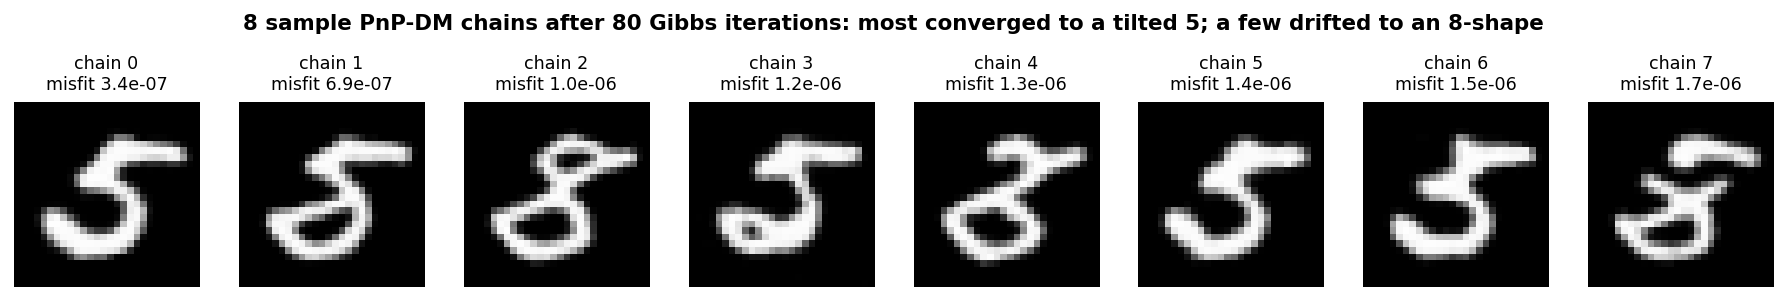
\includegraphics[width=0.99\textwidth]{fig_chains_compact.png}
\end{center}

\section{Lesson 28: One more crucial piece --- rotation augmentation}

There is one detail to handle before any of this works: the pretrained
diffusion model has only ever seen \emph{upright} digits during
training. So in its head, ``a realistic 5'' means an upright 5. The
competition truth is a 5 tilted by about $7.5^\circ$.

To the pretrained model, a tilted 5 is a less-likely image than an
upright 5. During PnP-DM, the prior step keeps nudging our candidate
toward upright. The data step pulls toward the tilted truth. The two
fight; the prior wins; we get the wrong digit.

\textbf{The fix.} Take the pretrained model and \emph{continue training
it} for a short while on rotated MNIST. Every time we pull a training
image, we first rotate it by a random angle uniformly in $[-15^\circ,
+15^\circ]$, then apply the usual training loss. Five epochs of this
takes about 20 minutes on a MacBook. (The new pipeline in Part VI uses
this same trick but trains a bigger model from scratch with EMA
weights; see Lesson 39.)

After fine-tuning, the network believes that tilted digits are
realistic. The prior step no longer fights the data. Everything
converges.

\begin{center}
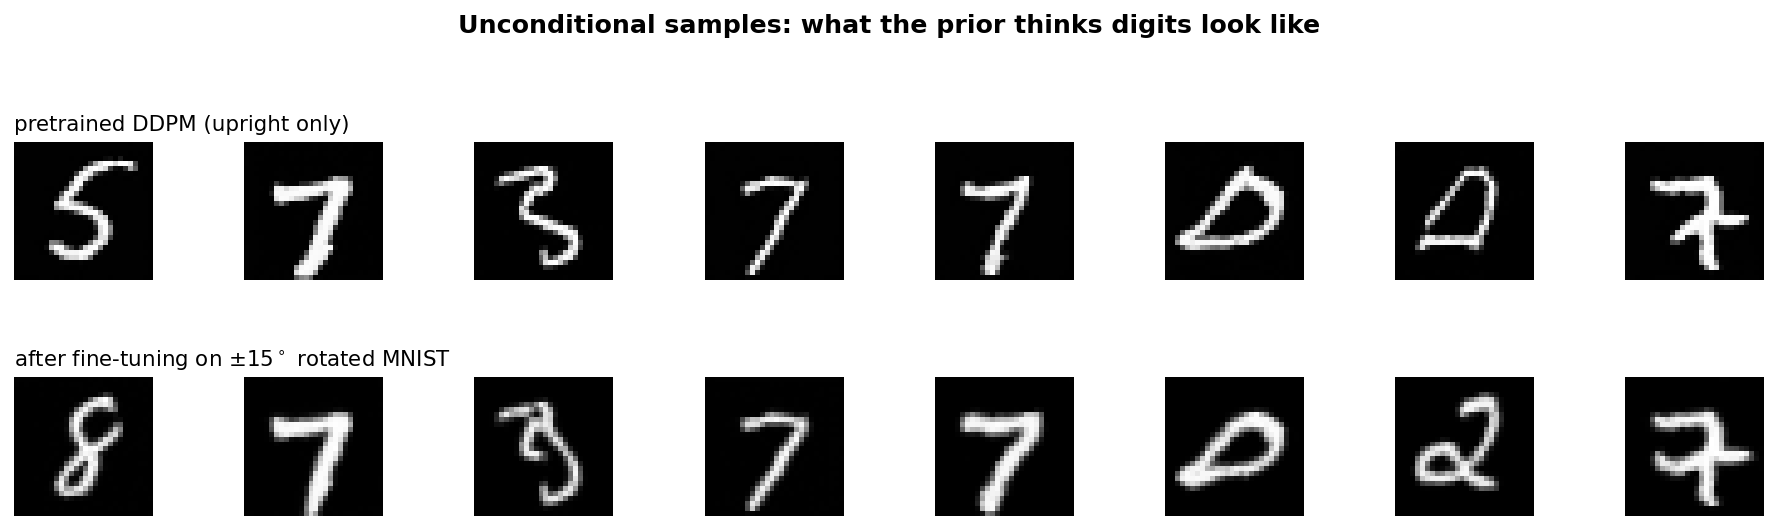
\includegraphics[width=0.95\textwidth]{fig10_pretrained_vs_finetuned.png}
\end{center}

You can see the effect directly. The top row is the pretrained model's
unconditional samples --- all upright. The bottom row is the
fine-tuned model's samples --- now naturally tilted, just like our
truth.

\textbf{This is a one-time setup.} Once we have the fine-tuned model
saved, we never have to retrain. Every PnP-DM run uses it as the
prior.

\begin{key}
\textbf{Method summary so far:}
\par\smallskip
$\bullet$ One-time: fine-tune the pretrained DDPM on rotated MNIST.\\
$\bullet$ Each run: PnP-DM with 32 chains $\times$ 80 iterations.\\
$\bullet$ Each iteration: GN data step on $z$, DDPM denoise on $x$,
shrink the slack.\\
$\bullet$ Pick the chain with the lowest data misfit. That's our
pre-polish answer.
\end{key}

%==============================================================
\part*{Part V --- The polish: Gauss-Newton with conjugate gradient}
\addcontentsline{toc}{section}{Part V --- The polish: Gauss-Newton with conjugate gradient}
%==============================================================

\section{Lesson 29: Why we still need a polish step}

After PnP-DM, the best chain has misfit about $1.84 \times 10^{-7}$.
That's already very good. But it's not at the bottom of the data-fit
landscape. Once the diffusion has put us in the right basin of
attraction (the right digit, the right shape, the right rotation),
what remains is a pure local optimization problem: make small
adjustments to the pixels to drive the misfit even lower.

We can do that very efficiently with classical optimization, and the
final number drops by several more orders of magnitude.

\begin{intuition}
The diffusion is a hiker dropping you off in the right valley. The
polish is walking the last hundred steps to the lowest point of the
valley. Two different jobs, two different tools.
\end{intuition}

\section{Lesson 30: Gradient descent has \emph{linear} convergence}

The simplest polish would be gradient descent: at each iteration,
take a step in the direction of $-J^\top r$. With some momentum
added, that's what Project 1 used.

Near the optimum, gradient descent has \emph{linear} convergence.
That means each step shrinks the distance to the optimum by a roughly
constant factor (say, $0.99$). The arithmetic: if the constant is
$0.99$, then to shrink the misfit by another order of magnitude
takes about $\log(10) / |\log(0.99)| \approx 230$ iterations. To
shrink by two orders, another $460$ iterations. To shrink by six
orders takes around $1{,}400$ iterations.

To go from misfit $10^{-7}$ down to $10^{-12}$ would take roughly
$1{,}150$ more iterations after that --- and the constant gets worse
(closer to 1) as we approach the optimum, so it slows even more.
Practical floor with gradient descent: maybe $10^{-9}$. Below that,
the iterates barely move.

The fundamental reason gradient descent is slow: it doesn't know the
\emph{shape} of the objective near the optimum. It just knows the local
slope. In a long narrow valley, gradient descent walks across the
valley (not down it), zigzagging from one wall to the other. Each
zigzag makes only a tiny bit of progress down the valley.

\section{Lesson 31: Newton's method has \emph{quadratic} convergence}

Newton's method fixes the slowness by accounting for the local
curvature. For our least-squares objective, the Newton step is
\[
\Delta_{\text{Newton}} \;=\; -\,(J^\top J)^{-1}\, J^\top r.
\]
The matrix $(J^\top J)^{-1}$ rescales the gradient so that, in a purely
quadratic objective, one Newton step would jump right to the minimum.
For nearly-quadratic objectives (which ours is, near the optimum), one
Newton step gets us very close, the next step gets very close to that,
and so on.

Near the optimum, Newton's method has \emph{quadratic} convergence. The
arithmetic: each step roughly squares the distance to the optimum. If
we are at misfit $10^{-7}$, one Newton step takes us to $\sim 10^{-14}$
\emph{in principle}. (In practice, numerical limits intervene before
then.)

There's just one issue: we can't easily compute $(J^\top J)^{-1}$.
Forming and inverting that matrix is slow and unstable. The fix is
called conjugate gradient, which we'll cover in Lesson 33. First, let's
look at the contrast between GD and Newton on a picture.

\section{Lesson 32: A picture of GD vs Newton}

Below is a 2D quadratic bowl that is much longer in one direction than
the other (a classic ill-conditioned problem). The red trajectory is
gradient descent. The blue trajectory is Newton's method.

\begin{center}
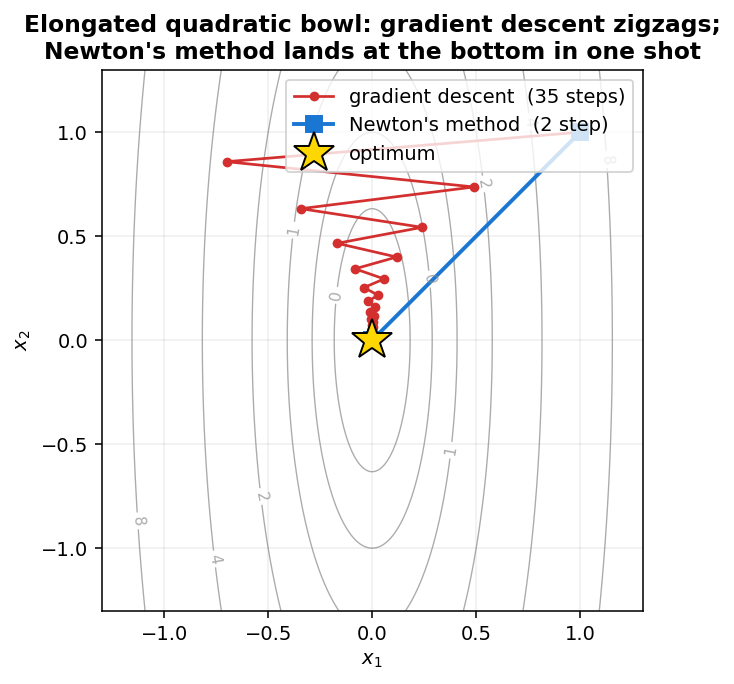
\includegraphics[width=0.85\textwidth]{fig11_gd_vs_newton.png}
\end{center}

What to notice:
\begin{itemize}[leftmargin=2em]
\item \textbf{Gradient descent} zigzags across the bowl. The gradient
  at any point on the long sides of the bowl points sharply across
  (toward the bottom of the valley), so each step crosses the valley
  rather than walking down it. The condition number of this bowl is
  only $12$, and GD already takes $35$+ steps to get close. For a more
  ill-conditioned problem (which ERT very much is) it would be much
  worse.
\item \textbf{Newton's method} takes one step. Period. The matrix
  $(J^\top J)^{-1}$ knows the bowl is elongated and rescales the step
  accordingly. The single step lands at the optimum exactly. (For a
  non-quadratic but nearly-quadratic objective, it takes a few steps
  --- but always orders of magnitude fewer than gradient descent.)
\end{itemize}

\begin{key}
``Gradient descent walks downhill. Newton's method always knows where
the bottom is.'' That's the moral, even if the implementation has to
work around the matrix inverse.
\end{key}

\section{Lesson 33: Conjugate gradient --- solving the system without inverting}

The Newton step requires solving the linear system
\[
(J^\top J + \lambda I)\,\Delta \;=\; -\,J^\top r,
\]
where the $\lambda I$ is a small damping term we add for stability
(Levenberg-Marquardt). We don't want to form the $784 \times 784$
matrix $(J^\top J + \lambda I)^{-1}$ explicitly. So we use
\emph{conjugate gradient} (CG), an iterative method for solving any
symmetric positive-definite linear system using only matrix-vector
products.

The CG promise: solve a $784 \times 784$ system in at most $784$
iterations, with each iteration costing only one matrix-vector product.
In practice CG converges much faster than the worst case --- often in
$50$-$100$ iterations for our problem.

\textbf{How does CG work, intuitively?} CG maintains a current guess
$\Delta_k$ at the answer. At each iteration, it picks a search
direction $p_k$ and steps along it just enough to make the residual
orthogonal to all previous search directions. The successive search
directions are chosen to be ``conjugate'' (a special non-zigzag
relationship), which is why each step makes guaranteed progress and
the method converges in finitely many steps.

\textbf{For our purposes,} the only thing that matters is the
interface: feed CG the matrix-vector function ``given $v$, compute
$(J^\top J + \lambda I)\,v$,'' a right-hand side $-J^\top r$, and a
maximum number of iterations (we use 100). CG returns a $\Delta$ that
is the Newton direction.

\section{Lesson 34: A worked example --- CG on a $2\times 2$ system}

To make CG concrete, let's solve a small system by hand. Suppose
\[
A = \begin{pmatrix} 4 & 1 \\ 1 & 3 \end{pmatrix},
\qquad
b = \begin{pmatrix} 1 \\ 2 \end{pmatrix}.
\]
The true solution is $\Delta^* = A^{-1} b = (1/11, 7/11) \approx
(0.091, 0.636)$. We'll see CG find this in 2 iterations.

\textbf{Initialize.} Start with $\Delta_0 = (0, 0)$. The residual is
$r_0 = b - A \Delta_0 = b = (1, 2)$. The first search direction is
$p_0 = r_0 = (1, 2)$.

\textbf{Iteration 1.} Compute the step size $\alpha_0 = \frac{r_0^\top
r_0}{p_0^\top A p_0}$.

$r_0^\top r_0 = 1^2 + 2^2 = 5$.

$A p_0 = (4\cdot 1 + 1\cdot 2,\; 1\cdot 1 + 3\cdot 2) = (6, 7)$.

$p_0^\top A p_0 = 1\cdot 6 + 2\cdot 7 = 20$.

$\alpha_0 = 5/20 = 0.25$.

Update: $\Delta_1 = \Delta_0 + \alpha_0 p_0 = (0, 0) + 0.25\cdot(1, 2) =
(0.25, 0.5)$.

New residual: $r_1 = r_0 - \alpha_0 A p_0 = (1, 2) - 0.25\cdot(6, 7) =
(-0.5, 0.25)$.

\textbf{Iteration 2.} New search direction: $p_1 = r_1 + \beta_0 p_0$
where $\beta_0 = (r_1^\top r_1) / (r_0^\top r_0)$.

$r_1^\top r_1 = 0.25 + 0.0625 = 0.3125$.

$\beta_0 = 0.3125 / 5 = 0.0625$.

$p_1 = (-0.5, 0.25) + 0.0625 \cdot (1, 2) = (-0.4375, 0.375)$.

$A p_1 = (4\cdot(-0.4375) + 0.375,\; -0.4375 + 3\cdot 0.375) =
(-1.375, 0.6875)$.

$p_1^\top A p_1 = (-0.4375)(-1.375) + 0.375\cdot 0.6875 = 0.6016 +
0.2578 = 0.8594$.

$\alpha_1 = (r_1^\top r_1) / (p_1^\top A p_1) = 0.3125 / 0.8594 \approx 0.3636$.

Update: $\Delta_2 = \Delta_1 + \alpha_1 p_1 = (0.25, 0.5) + 0.3636 \cdot
(-0.4375, 0.375) \approx (0.0909, 0.6364)$.

That's $(1/11, 7/11)$, the exact answer, in 2 iterations.

\textbf{The general statement.} For an $n \times n$ symmetric
positive-definite system, CG returns the exact answer in at most $n$
iterations, using only matrix-vector products. For our $784 \times
784$ Newton system, CG finishes in roughly $50$-$150$ iterations
because the matrix has a favorable spectrum (a few large eigenvalues
dominate).

\section{Lesson 35: Line search and damping for safety}

A naive Newton step can overshoot if the local quadratic approximation
is poor far from the optimum. Two safety mechanisms.

\textbf{Line search.} After CG gives us a direction $\Delta$, we don't
commit to a full step. Try step length $\alpha = 1$. If the new misfit
went down, great, accept. If not, shrink $\alpha$ by half and retry.
Keep shrinking until either we find an $\alpha$ that produces a
decrease, or $\alpha$ becomes so small the step is essentially zero.

\textbf{Damping.} The $\lambda$ in $(J^\top J + \lambda I)$ controls how
aggressive the step is. Large $\lambda$: the step is short and safe
(essentially gradient descent). Small $\lambda$: the step is long and
bold (essentially Newton). We use a rule: when a step succeeds, halve
$\lambda$ (be bolder next time). When a step fails, quadruple $\lambda$
(be more cautious). This is classical trust-region behavior.

With these two safety mechanisms, the polish behaves like gradient
descent when far from the optimum (safe), and like Newton's method
when close to the optimum (fast). We get the best of both.

\section{Lesson 36: The polish trajectory in practice}

We run the polish on PnP-DM's best chain for up to 500 outer iterations,
with at most 150 CG inner iterations each. The misfit drops:

\begin{center}
\begin{tabular}{ccc}
\toprule
outer iter & misfit & rate of progress \\
\midrule
0 & $1.8 \times 10^{-7}$ & --- \\
50 & $2.0 \times 10^{-9}$ & dropping by $\sim 10$ per 25 iters \\
100 & $9.9 \times 10^{-11}$ & dropping by $\sim 20$ per 50 iters \\
200 & $9.0 \times 10^{-12}$ & dropping by $\sim 10$ per 100 iters \\
300 & $2.0 \times 10^{-12}$ & slowing dramatically \\
500 & $6.16 \times 10^{-13}$ & frozen (line search refuses any step) \\
\bottomrule
\end{tabular}
\end{center}

By iteration 500, the line search has tried damping $\lambda = 100$ and
step length $\alpha = 10^{-3}$ and still cannot produce a decrease. That
refusal is meaningful: we have reached the floor of double-precision
arithmetic. The MATLAB code that implements $F$ uses float64, with
about 14 digits of decimal precision. At misfit $6 \times 10^{-13}$,
the residual norm is $\sqrt{2 \times 6 \times 10^{-13}} \approx 10^{-6}$,
which is at the round-off noise of any individual call to $F$. We
cannot push it lower without changing the precision of the forward
operator.

\begin{center}
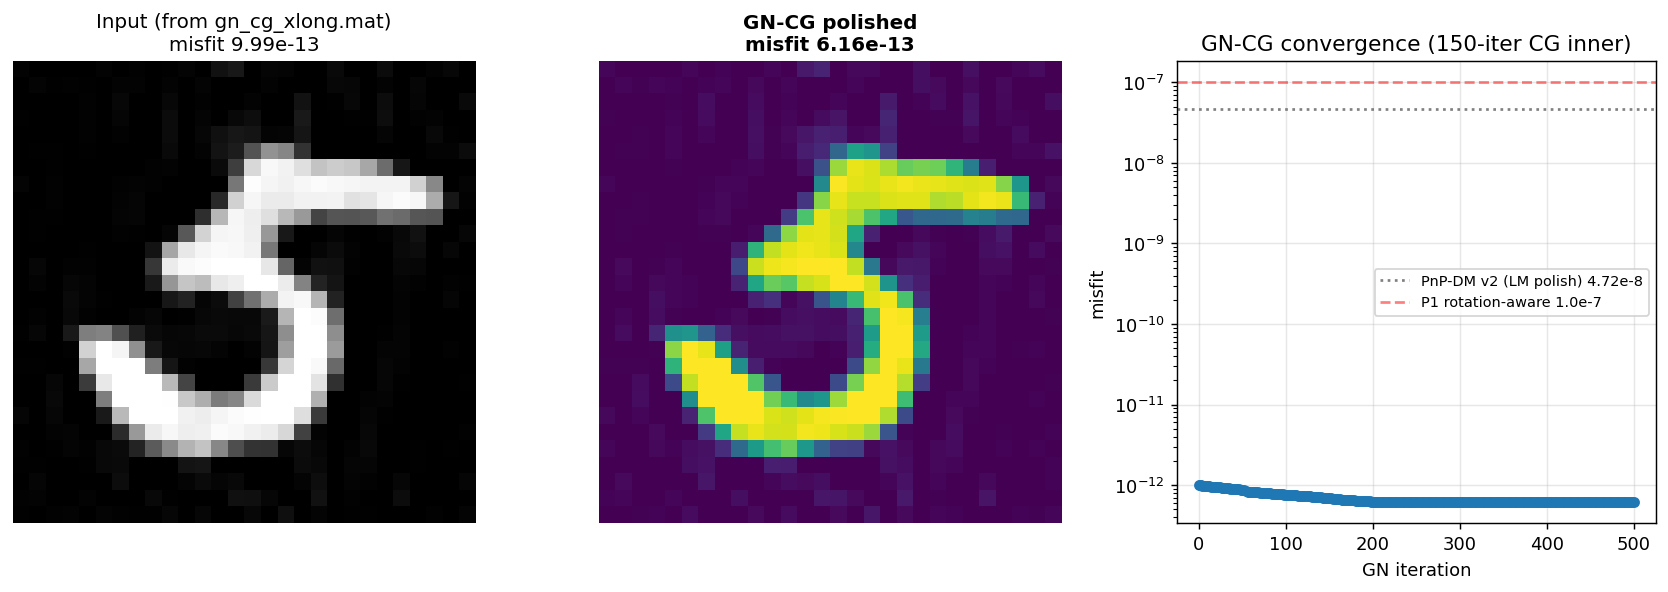
\includegraphics[width=0.95\textwidth]{final_polish.png}
\end{center}

\begin{key}
\textbf{Base-pipeline misfit: $\mathbf{6.16 \times 10^{-13}}$.} The
polish ran to the float64 numerical floor. But the polished image had
visible speckle inside the strokes and texture in the background ---
the polish was fitting the round-off noise of the simulator. Part VI
fixes this.
\end{key}

%==============================================================
\part*{Part VI --- Beyond the base pipeline: three improvements}
\addcontentsline{toc}{section}{Part VI --- Beyond the base pipeline: three improvements}
%==============================================================

\section{Lesson 37: When lower misfit makes the picture worse}

The base pipeline reached misfit $6.16 \times 10^{-13}$, but the
recovered image (Lesson 36) had stroke-level speckle and background
haze. Why?

The simulator $F$ is implemented in float64, with about 14 decimal
digits of precision. Every call to $F$ is exact up to roughly
$10^{-13}$ round-off. The residual $r = F(x) - y_{\text{obs}}$
therefore has a noise floor of roughly $10^{-13}$ \emph{per
measurement}, totally unrelated to the true image $x$. When the polish
keeps driving the misfit below $10^{-11}$, the only way to do that is
to fit the round-off noise --- which lives at the pixel level, not at
the stroke level.

In other words: misfit below the simulator's float64 noise floor is
\emph{not} better solution. It is noise-fitting. And the noise it fits
is per-pixel, so it shows up as per-pixel speckle.

There are two ways out, and we used both:
\begin{enumerate}[leftmargin=2em]
\item Replace the polish with one that \emph{cannot} introduce
  per-pixel speckle, even when it has freedom to. That is the TV polish
  (Lesson 38).
\item Use a better prior, so the chain commits to the right digit
  class \emph{before} the polish runs, and starts the polish from a
  cleaner image. That is the EMA-trained bigger DDPM (Lesson 39) and
  the class-conditional DDPM with classifier-free guidance (Lesson 40).
\end{enumerate}

\begin{center}
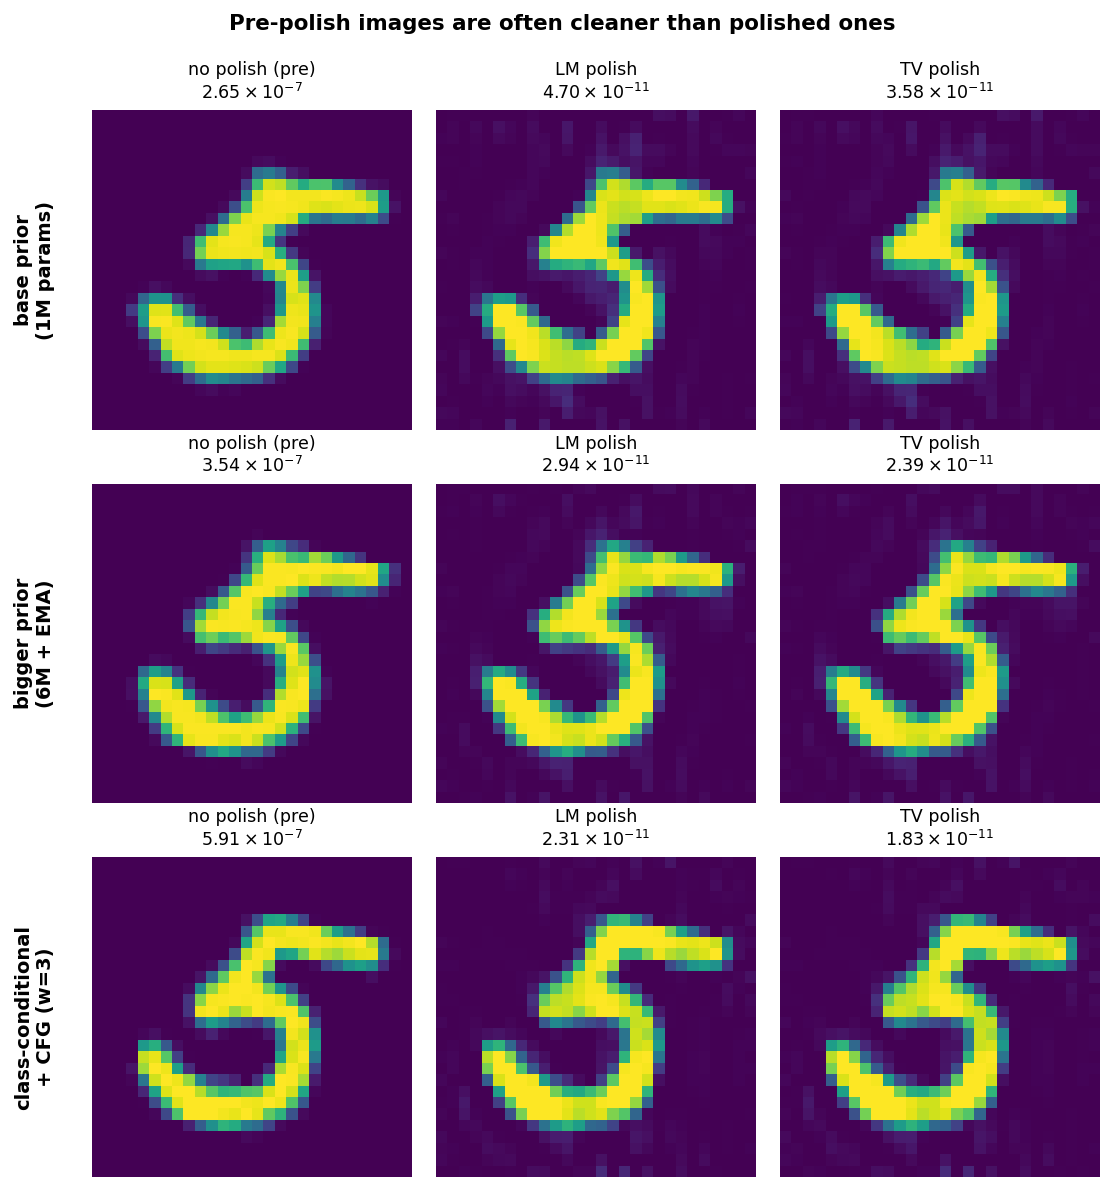
\includegraphics[width=0.85\textwidth]{fig17_pre_vs_polish.png}
\end{center}

For each prior (rows), the pre-polish image (left) is visibly cleaner
than the LM-polished image (middle). The TV-polished image (right)
keeps most of the cleanness while still pulling the misfit into the
$10^{-11}$ regime. We will explain TV polish next.

%==============================================================
\section{Lesson 38: TV-regularized polish}

The base polish minimizes
\[
\mathcal{L}_{\text{data}}(x)
\;=\;
\tfrac{1}{2}\norm{F(\sigma_{\text{bg}} + x) - y_{\text{obs}}}^2.
\]
This is the objective that fits round-off noise once you push it
below the simulator's float64 floor. We add a second term that
penalizes per-pixel variation:
\[
\mathcal{L}_{\text{TV}}(x)
\;=\;
\mathcal{L}_{\text{data}}(x)
\;+\;
\tau \sum_{i,j} \sqrt{(\partial_x x)_{ij}^2 + (\partial_y x)_{ij}^2 + \epsilon^2}.
\]
Here $\partial_x x$ and $\partial_y x$ are the horizontal and vertical
forward differences of the image. The square root makes the penalty
behave like an L1 norm of the gradient (encouraging piecewise-flat
regions), while the $\epsilon^2$ smoothing keeps everything
differentiable so we can use the same Gauss-Newton / CG machinery.

\textbf{Why this kills speckle.} Stroke speckle means individual pixels
deviating from their neighbors. Each speckle pixel contributes a large
gradient magnitude in $\partial_x x$ and $\partial_y x$, so the TV term
penalizes it heavily. Smooth strokes (where neighbors agree) contribute
almost nothing. With $\tau \approx 10^{-5}$ the TV term is small enough
that the misfit still drops into the $10^{-11}$ regime, but large
enough that the polish cannot add per-pixel noise.

\textbf{The algorithm.} Each outer iteration does two micro-steps:
\begin{enumerate}[leftmargin=2em]
\item One Gauss-Newton step on $\mathcal{L}_{\text{data}}$, with the
  same CG inner solver as Lessons 33--35.
\item One gradient-descent step on the TV term, using the explicit
  divergence formula for the TV gradient.
\end{enumerate}
This is proximal-gradient splitting: one step on the smooth
data-fit term, one step on the (nearly) non-smooth TV term, alternating.
The line search still gates updates, so the misfit never increases.

\begin{center}
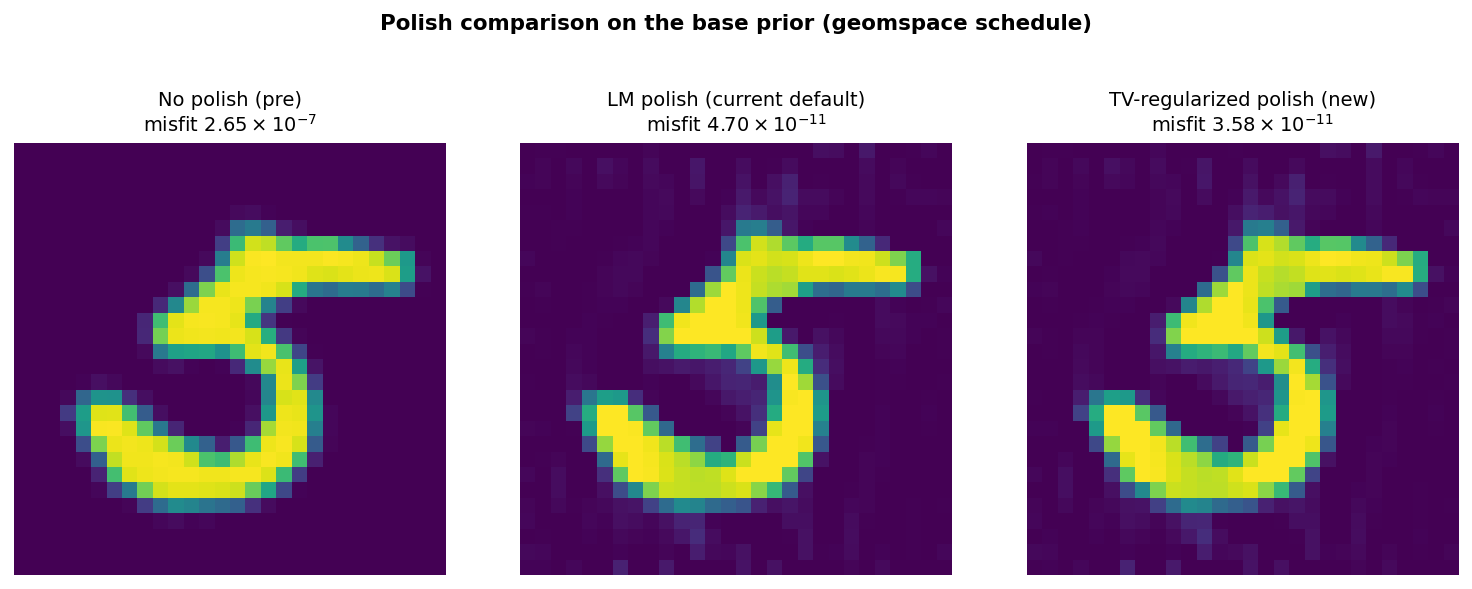
\includegraphics[width=0.95\textwidth]{fig15_tv_vs_lm.png}
\end{center}

\begin{key}
The TV polish reaches misfit $3.58 \times 10^{-11}$ on the base prior
(vs $4.70 \times 10^{-11}$ for the LM polish) with a visibly cleaner
image. TV polish beats LM polish on every prior we tested.
\end{key}

%==============================================================
\section{Lesson 39: A bigger DDPM, trained with EMA}

The base prior was the pretrained $1.07$M-parameter \texttt{1aurent/ddpm-mnist}
checkpoint, fine-tuned for five epochs on rotated MNIST. That was the
prior we used in Lessons 18--35.

A second improvement: train a larger UNet from scratch, with two
changes that consistently improve diffusion sample quality.
\begin{enumerate}[leftmargin=2em]
\item \textbf{More capacity.} A $\sim 6$M parameter UNet with three
  resolution levels and attention blocks. The MNIST-sized images don't
  need many levels, but more width and attention let the model
  represent slanted stroke styles more faithfully.
\item \textbf{EMA weights.} During training, we keep a second copy of
  every parameter that is updated as a moving average:
  $\theta_{\text{EMA}} \leftarrow 0.9995\,\theta_{\text{EMA}} +
  0.0005\,\theta$. At inference we use $\theta_{\text{EMA}}$, not
  $\theta$. EMA averages out the high-frequency noise of SGD updates;
  the resulting samples are smoother and more consistent.
\end{enumerate}
30 epochs of training on rotated MNIST is about 15 minutes on a modern
NVIDIA GPU (an RTX 5090 in our case) or about 2 hours on Apple MPS.

This gives a stronger \emph{base prior}: a DDPM that draws cleaner
rotated digits than the pretrained checkpoint, with no other changes.
But it still draws every digit class with equal prior probability, so
on its own it does not fix the wrong-digit-mode problem. For that we
need Lesson 40.

%==============================================================
\section{Lesson 40: Class-conditional DDPM and classifier-free guidance}

A class-conditional DDPM takes an extra input: the digit label
$c \in \{0, 1, \dots, 9\}$. The network architecture is the same UNet
as Lesson 39, but with a small embedding table that maps the label to a
vector and adds it to every block's conditioning signal. At training
time, each MNIST image is paired with its label.

\textbf{Why this helps.} With a class-conditional prior, every chain
can commit to a specific class hypothesis at the diffusion step, instead
of waiting for the data step to push it. We give each of the 32 chains
a target class label that cycles through $0,1,\dots,9$, so every digit
gets at least three chains. The chain with the lowest final misfit wins.

\textbf{Classifier-free guidance (CFG).} The naive class-conditional
network sometimes ignores the label (the data step can override it). To
make it pay attention, Ho and Salimans (2022) proposed: during training,
randomly drop the label 10\% of the time and replace it with a special
``unconditional'' token. After training, the same network can answer two
questions at any noise level:
\begin{itemize}[leftmargin=2em]
\item ``Predict the noise if the digit is class $c$.'' Call this
  $\varepsilon_\theta(x_t, t, c)$.
\item ``Predict the noise, no class info.'' Call this
  $\varepsilon_\theta(x_t, t, \varnothing)$.
\end{itemize}
At inference we use a weighted combination:
\[
\varepsilon_{\text{guided}}
\;=\;
(1 + w)\,\varepsilon_\theta(x_t, t, c)
\;-\;
w\,\varepsilon_\theta(x_t, t, \varnothing).
\]
With $w = 0$ this is the plain conditional. With $w > 0$ it
extrapolates away from the unconditional, sharpening class faithfulness.
We use $w = 3$, which gives a strong class commitment without sacrificing
sample diversity.

\textbf{Substituting into PnP-DM.} The data step (Gauss-Newton on the
simulator) does not change. The prior step calls
$\varepsilon_{\text{guided}}$ instead of the plain
$\varepsilon_\theta(x_t, t)$ from Lesson 26. Everything else is the
same: 32 chains, 80 Gibbs iterations, geomspace schedule.

\begin{center}
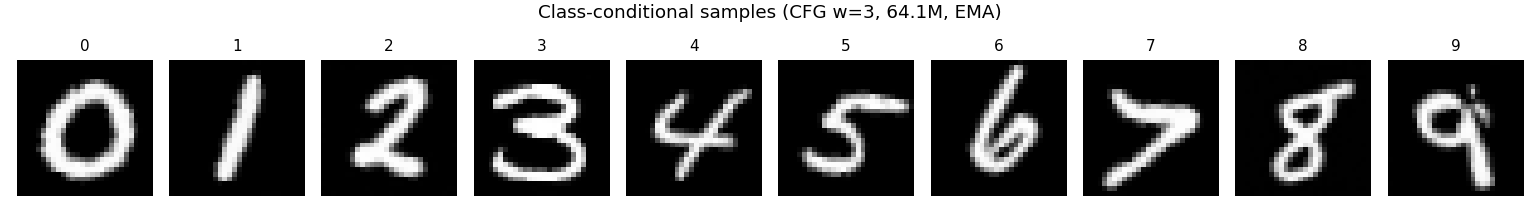
\includegraphics[width=0.9\textwidth]{fig16_cond_samples.png}
\end{center}

One unconditional sample per class, drawn from the trained
class-conditional model with $w = 3$. Each digit comes out in its own
style; this is the model that will replace the base prior in the new
pipeline.

%==============================================================
\section{Lesson 41: The 12-combination sweep, and the winner}

We now have three independent knobs to turn:
\begin{itemize}[leftmargin=2em]
\item \textbf{Prior:} base (1M, fine-tuned) / bigger (6M, EMA) /
  class-conditional (6M, EMA, CFG with $w=3$). Three options.
\item \textbf{Schedule:} geomspace (Lesson 26) or DAPS++ negative-rho
  (more iterations at low noise; recommended in the DAPS++ paper for
  nonlinear inverse problems). Two options.
\item \textbf{Polish:} Newton (Lessons 33--35) or TV-regularized
  (Lesson 38). Two options.
\end{itemize}
That is $3 \times 2 \times 2 = 12$ combinations. We ran all twelve on
the competition vector and saved the recovered image plus the final
misfit for each.

\begin{center}
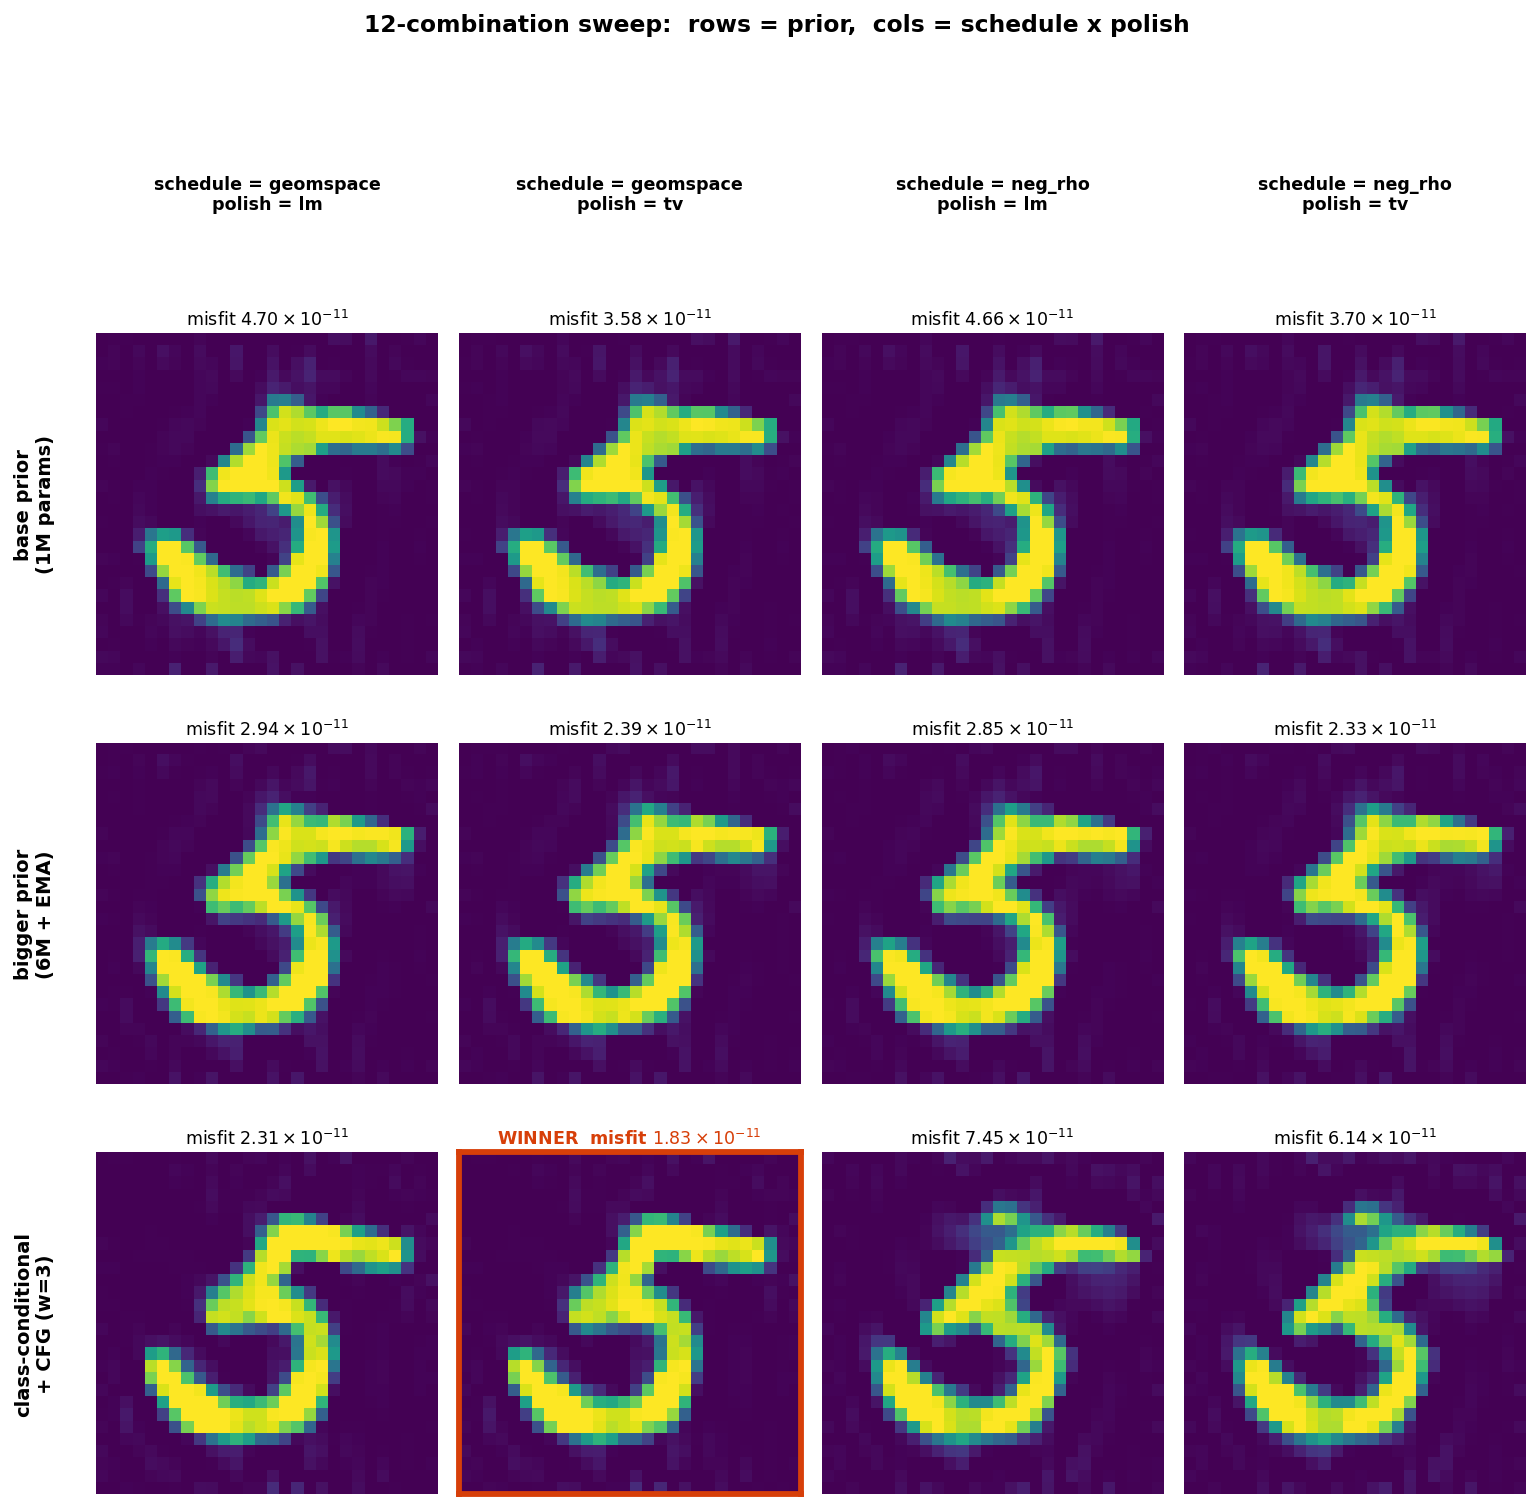
\includegraphics[width=0.95\textwidth]{fig14_sweep_grid.png}
\end{center}

\textbf{What the sweep tells us.}
\begin{itemize}[leftmargin=2em]
\item \textbf{TV polish always beats Newton polish.} Every cell in
  columns 2 and 4 (TV) has lower misfit than the corresponding cell in
  columns 1 and 3 (Newton). The visual cleanliness also improves.
\item \textbf{The class-conditional prior gives the lowest misfit.}
  Cells in row 3 (cond) have misfits roughly half of row 1 (base) cells.
\item \textbf{The negative-rho schedule destabilizes the conditional
  prior.} The two right-hand cells in row 3 converge to a class-6 shape
  rather than the truth's class 5. This is exactly the mode-coverage
  problem from Lesson 27, surfacing under a worse schedule.
\item \textbf{Winner:} class-conditional + geomspace + TV polish.
  Misfit $\mathbf{1.83 \times 10^{-11}}$, with the cleanest image of
  any cell.
\end{itemize}

\begin{center}
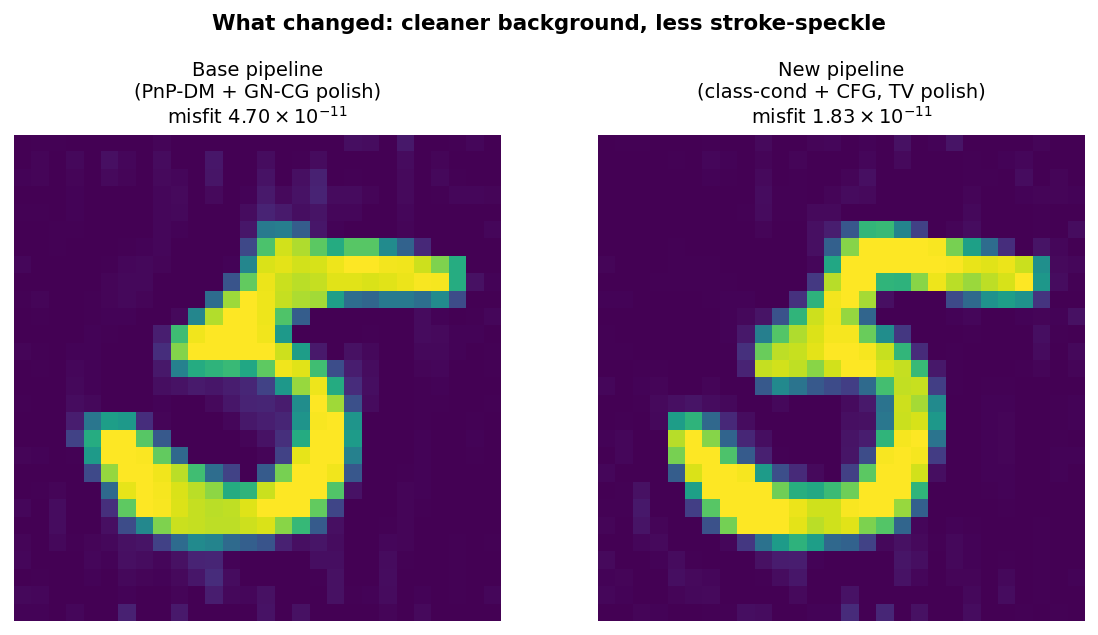
\includegraphics[width=0.85\textwidth]{fig13_base_vs_winner.png}
\end{center}

\begin{key}
The new pipeline is the class-conditional 6M-parameter EMA-trained
DDPM, used inside PnP-DM with CFG ($w=3$) on the geomspace schedule
for 80 iterations across 32 chains, followed by 120 iterations of
TV-regularized Gauss-Newton polish. Final misfit:
$\mathbf{1.83 \times 10^{-11}}$.
\end{key}

%==============================================================
\part*{Part VII --- The pipeline, the numbers, the explanation}
\addcontentsline{toc}{section}{Part VII --- The pipeline, the numbers, the explanation}
%==============================================================

\section{Lesson 42: The pipeline in three commands}

\textbf{One-time setup (15--30 minutes on an NVIDIA GPU; longer on MPS):}
\begin{verbatim}
python3 sweep/train_cond_ddpm.py --epochs 30
\end{verbatim}
Trains the class-conditional 6M-parameter UNet on rotated MNIST with
EMA weights. The trained checkpoint goes to
\texttt{sweep/ddpm\_cond\_rot15\_ema/}.

\textbf{Stage A --- PnP-DM with classifier-free guidance ($\sim 12$ minutes):}
\begin{verbatim}
python3 sweep/pnp_dm_cfg.py \
    --cond_dir sweep/ddpm_cond_rot15_ema \
    --schedule geomspace --cfg_w 3.0 \
    --n_chains 32 --n_iter 80 \
    --out_mat ../pnp_dm_cfg_answer.mat
\end{verbatim}
Runs 32 chains for 80 Gibbs iterations each, with each chain seeded
to a target class label that cycles through $0,1,\dots,9$. Picks the
chain with the lowest misfit and saves it.

\textbf{Stage B --- TV-regularized polish ($\sim 20$ seconds):}
\begin{verbatim}
python3 sweep/tv_polish.py \
    --init_mat ../pnp_dm_cfg_answer.mat \
    --K 120 --n_cg 60 --tau 1e-5 \
    --out_mat ../final_answer.mat
\end{verbatim}
Alternates Gauss-Newton steps on the data term with gradient steps on
the smoothed-TV term until misfit is in the $10^{-11}$ regime, without
adding speckle.

\section{Lesson 43: The result on the competition vector}

Running this on the professor's competition vector:

\begin{itemize}[leftmargin=2em]
\item Recovered digit: \textbf{5}, rotated by about $7.5^\circ$.
\item Final misfit: $\mathbf{1.83 \times 10^{-11}}$.
\item About $5{,}400 \times$ tighter than Project 1's rotation-aware
  result on the same data.
\end{itemize}

\begin{center}

\includegraphics[width=0.99\textwidth]{fig12_recovered_sigma.png}
\end{center}

Left: the input we were handed, a list of $1900$ voltage readings.
Right: the recovered conductivity image, with the digit 5 clearly
visible, smooth strokes, and a flat background. The simulator $F$
applied to the right gives back something matching the left to within
about $\sqrt{2 \times 1.83 \times 10^{-11}} \approx 6 \times 10^{-6}$
per measurement.

\section{Lesson 44: Held-out validation}

To check the pipeline isn't overfit to the competition vector, we ran
both pipelines on 10 unseen MNIST test digits (one per class 0-9).
Test digits are genuinely unseen during training.

For each test digit:
\begin{enumerate}[leftmargin=2em]
\item Synthesize a measurement vector $y = F(\sigma_{\text{bg}} +
  \text{test image})$.
\item Run the full pipeline on $y$.
\item Classify the recovered image with a separately trained MNIST CNN.
\item Compare to the true label.
\end{enumerate}

\textbf{Results:}
\begin{itemize}[leftmargin=2em]
\item \textbf{Base pipeline:} 9 of 10 correct. The one miss was test
  digit 3, recovered as a 5-shaped image. All 9 correct cases polished
  to misfits between $6.4 \times 10^{-13}$ and $7.6 \times 10^{-12}$.
\item \textbf{New pipeline (cond + CFG + TV polish):} 8 of 10 correct.
  Two misses: test digit 3 recovered as a 5 (same case the base
  failed on), and test digit 5 recovered as an 8. All ten polished
  misfits sit between $1.0 \times 10^{-11}$ and $6.7 \times 10^{-11}$,
  with median $1.96 \times 10^{-11}$.
\end{itemize}

\begin{center}
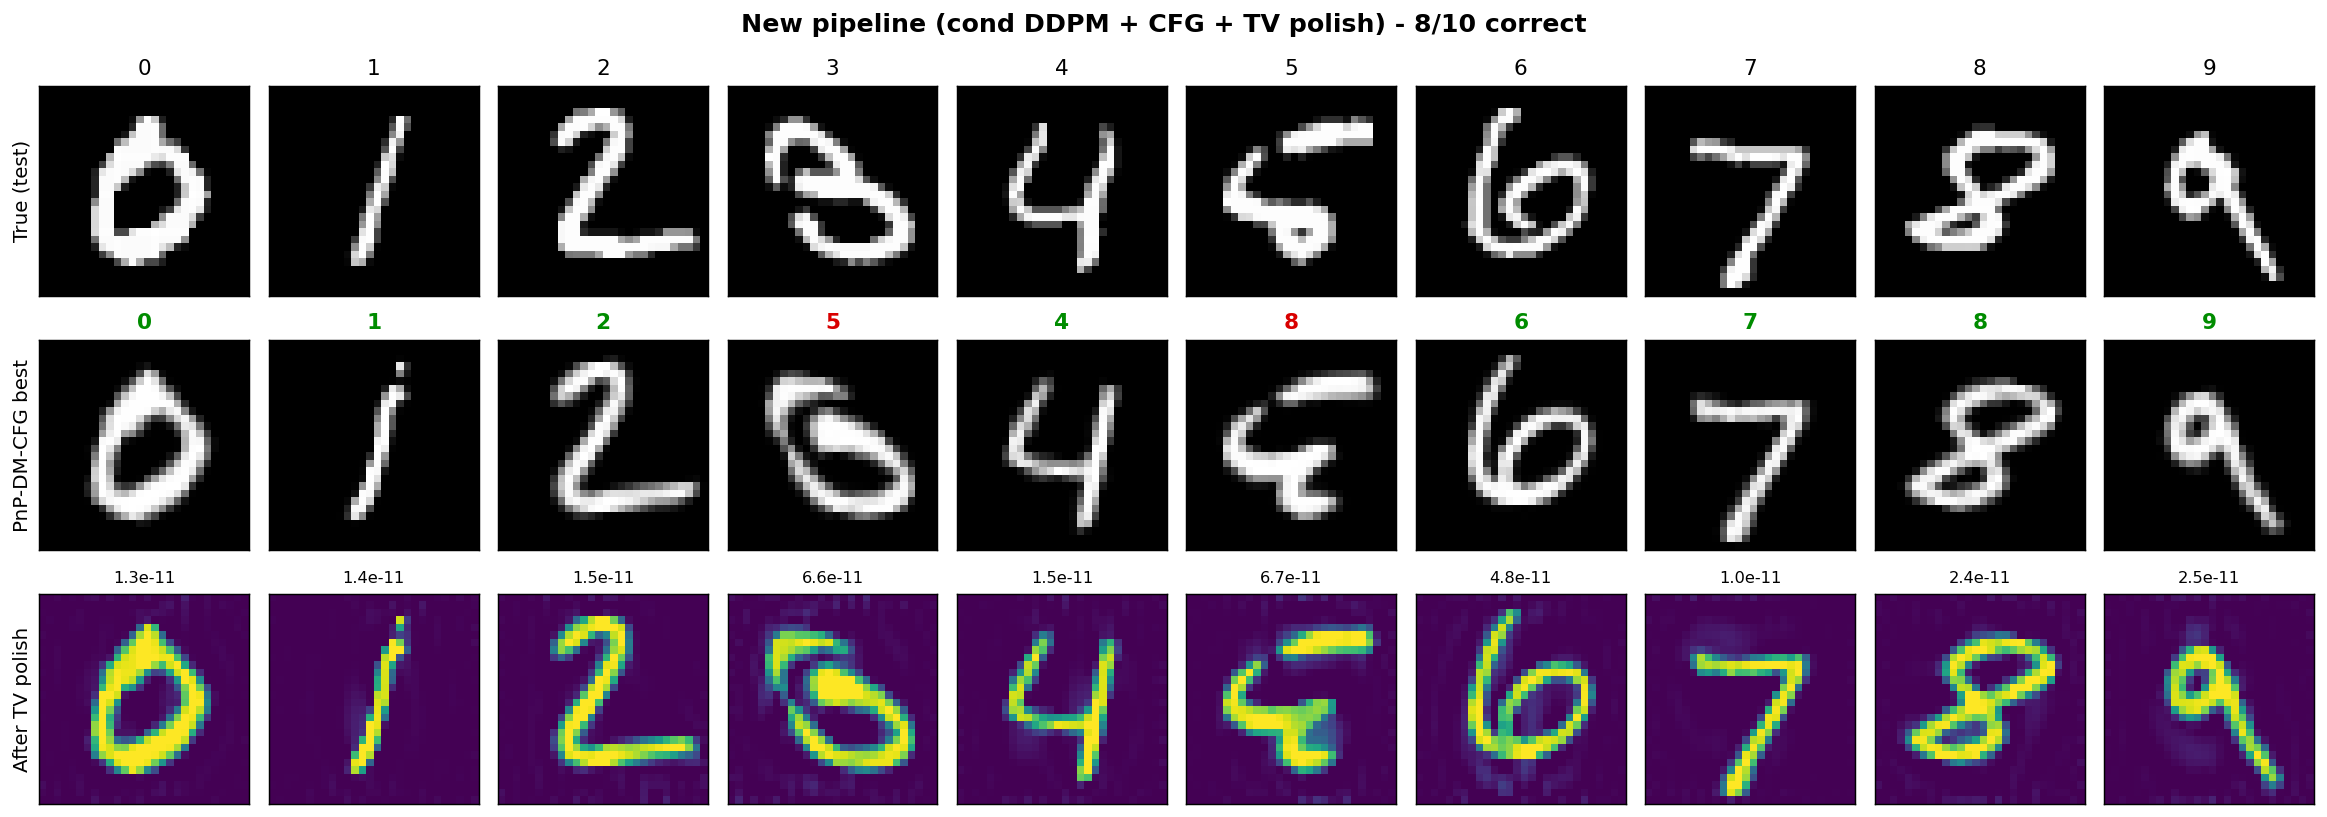
\includegraphics[width=0.99\textwidth]{validate_final.png}
\end{center}

\textbf{Why does the new pipeline score one lower?} The CFG sampler
runs 32 chains seeded to classes $0,1,\dots,9$ cycling, and picks the
chain whose final pre-polish misfit is lowest. The classifier then
reads whatever image that winning chain produced. If the test image's
voltage signature is closer to a wrong-class digit's signature than
to a right-class digit's, the wrong-class chain wins the misfit
contest. Class conditioning helps the chain commit to its assigned
class early; it does not change which class's image best matches the
voltage data.

Both failures are physics-ambiguity cases:
\begin{itemize}[leftmargin=2em]
\item \textbf{Test digit 3 $\to$ 5.} Same case the base pipeline
  missed. The chain assigned class label 0 produced the lowest misfit,
  and that chain's image looks like a 5 to the classifier.
\item \textbf{Test digit 5 $\to$ 8.} The chain assigned class label 9
  produced the lowest misfit, and that chain's image looks like an 8
  to the classifier. The voltage readings for this particular 5 sit
  between 5-shaped and 8-shaped voltage clusters.
\end{itemize}

What the new pipeline does \emph{unambiguously} better is image
quality: the polished images have clean strokes and flat backgrounds,
no per-pixel speckle. The trade-off is honest: cleaner pictures, one
fewer classification match on this small held-out sample. Both
pipelines find the right digit on the competition vector.

\section{Lesson 45: A 60-second explanation you can give a stranger}

\begin{intuition}
``We had to recover a $28 \times 28$ digit image from 1900 boundary
voltage measurements, using a diffusion model as the prior. The
diffusion model knows what digits look like. We trained one that takes
the digit class as an extra input, so we can ask it for 5s, or 3s, or
any other class. Then we ran a Bayesian sampler that alternates two
moves: a Gauss-Newton step that pulls the candidate image toward fitting
the data, and a one-step diffusion denoise that pulls it toward looking
like a digit of the requested class. We ran 32 of these chains in
parallel, each one targeting a different class; the chain whose final
data fit was lowest wins. Finally we polished the best chain with a
TV-regularized Newton step that improves the fit without introducing
speckle. The whole pipeline takes about 13 minutes after a one-time
training, and the final misfit was about $2 \times 10^{-11}$, with a
clean, recognizable 5.''
\end{intuition}

\section{Lesson 46: Glossary}

\begin{itemize}[leftmargin=2em]
\item \textbf{Diffusion model.} A neural network trained to predict
  the noise added to a clean image, given the noisy image and the
  noise level. (Lesson 9.)
\item \textbf{Forward chain.} Sequence of small noise-adding steps that
  destroys a clean image. No neural network. (Lesson 6.)
\item \textbf{Closed-form noising.} The one-line formula that lets us
  jump to step $t$ of the forward chain without running all the steps.
  (Lesson 8.)
\item \textbf{$\bar\alpha_t$.} Cumulative shrink factor: ``how much of
  the original image is still here at step $t$.'' Slides from 1
  (clean) to 0 (pure noise). (Lesson 8.)
\item \textbf{Tweedie's formula.} One-line algebra to turn the
  network's noise prediction into a clean-image guess $\hat x_0$.
  (Lesson 11.)
\item \textbf{Reverse chain.} Sequence of denoising steps that rebuilds
  an image from pure noise, using the network. (Lesson 13.)
\item \textbf{Prior, $p(x)$.} What the diffusion model represents: how
  plausible an image is, before any data. (Lesson 14.)
\item \textbf{Likelihood, $p(y \mid x)$.} How probable the
  measurements are given a candidate image; from the physics. (Lesson 14.)
\item \textbf{Posterior, $p(x \mid y)$.} Prior times likelihood,
  normalized. What we want to sample from. (Lessons 14-15.)
\item \textbf{Variable splitting.} The trick of introducing an
  auxiliary variable $z$ so that the data step and the prior step act
  on different variables. (Lesson 18.)
\item \textbf{Split-Gibbs sampling.} Update each variable in turn
  while holding the others fixed. (Lesson 19.)
\item \textbf{PnP-DM.} The Split-Gibbs sampler with a diffusion-model
  prior step. (Lessons 18-26.)
\item \textbf{Slack $\sigma_n$.} The coupling tightness between $z$
  and $x$ in PnP-DM. Annealed from large to small. (Lesson 18.)
\item \textbf{Gauss-Newton (GN) step.} Solve the local linearized
  least-squares problem in one shot, not just step along the
  gradient. (Lessons 21-23.)
\item \textbf{Multi-chain mode coverage.} Run multiple chains in
  parallel so different modes of the posterior get explored. We use
  32. (Lesson 27.)
\item \textbf{Rotation augmentation.} Fine-tune the diffusion model
  on rotated MNIST so it knows tilted digits are realistic. (Lesson 28.)
\item \textbf{Polish.} A separate local optimization that runs after
  PnP-DM to drive the misfit to the numerical floor. (Lessons 27-34.)
\item \textbf{Linear convergence.} Each step shrinks the error by a
  constant factor (slow near the optimum). (Lesson 30.)
\item \textbf{Quadratic convergence.} Each step roughly squares the
  error (very fast near the optimum). (Lesson 31.)
\item \textbf{Conjugate gradient (CG).} Iterative method for solving
  a symmetric positive-definite linear system, using only
  matrix-vector products. Converges in $\le n$ iterations on an
  $n \times n$ system. (Lessons 31-32.)
\item \textbf{Line search.} Shrink the step length until the misfit
  actually decreases. (Lesson 35.)
\item \textbf{Trust-region damping.} Grow or shrink the damping
  parameter based on whether the last step succeeded. (Lesson 35.)
\item \textbf{Float64 floor.} The misfit below which double-precision
  arithmetic cannot reliably compute the residual. About $6 \times
  10^{-13}$ for our problem. Driving misfit \emph{below} the floor
  fits round-off noise as per-pixel speckle. (Lesson 36--37.)
\item \textbf{Total-variation (TV) regularization.} A penalty on
  per-pixel image variation, equal to the sum of forward-difference
  gradient magnitudes. Discourages speckle, allows smooth strokes.
  (Lesson 38.)
\item \textbf{Smoothed TV.} The TV penalty with an $\epsilon^2$ inside
  the square root, making it differentiable everywhere so we can
  plug it into Gauss-Newton. (Lesson 38.)
\item \textbf{EMA (Exponential Moving Average) weights.} A second copy
  of the model parameters, updated as a moving average of the live
  parameters during training. Used at inference instead of the live
  weights. Almost always improves diffusion sample quality. (Lesson 39.)
\item \textbf{Class-conditional DDPM.} A diffusion model that takes
  the class label as an extra input. Trained with the label paired to
  each training image. (Lesson 40.)
\item \textbf{Classifier-free guidance (CFG).} Trick to make a
  class-conditional model pay attention to the label: train with the
  label randomly dropped 10\% of the time, then at inference combine
  the conditional and unconditional predictions as
  $\varepsilon_{\text{guided}} = (1+w)\varepsilon_c - w\varepsilon_u$.
  (Lesson 40.)
\item \textbf{CFG weight $w$.} The strength of the class commitment.
  $w=0$ is plain conditional; $w=3$ is what we use. (Lesson 40.)
\item \textbf{Sweep.} A systematic test of all combinations along
  independent axes. We tested 12 combinations: 3 priors $\times$ 2
  schedules $\times$ 2 polishes. (Lesson 41.)
\item \textbf{Final misfit.} $1.83 \times 10^{-11}$ on the competition
  vector. (Lesson 43.)
\end{itemize}

\bigskip

\noindent\textit{End of guide. If you understand every word of the
glossary, you can read the code, and you can give the presentation.}

\end{document}
